\chapter{Referencial Teórico}
\label{cap:referencial-teorico}

Neste capítulo serão apresentados os assuntos considerados fundamentais para o entendimento dos processos que estão envolvidos no uso das tecnologias abordadas no decorrer do trabalho. No início será discutida a criação dos shaders e seu uso ao longo do tempo, em seguida serão expostos itens de ordem técnica sobre os shaders e os motores de jogo. Ao final será tratada a integração dessas tecnologias com os processos de otimização.

\section{Evolução da Programação de Shaders}
\label{sec:historia-evolucao-programacao-shaders}

As representações visuais feitas através de imagens foram e são até hoje uma característica importante da formação da humanidade. Através do sentido da visão conseguimos absorver informações rapidamente, fazer associações durante o aprendizado e o estudo, ou ainda distinguir se algo é visualmente agradável o suficiente ou não para prender nossa atenção (LUTEN, 2014)\nocite{openGLBook}.

Os primeiros computadores tiveram seu acesso destinado a um público restrito devido aos custos elevados e a logística complexa. A forma de representação visual para os humanos dos pulsos elétricos gerados pelo seu processamento de dados era feita através de várias lâmpadas conectadas em placas ou de cartões de papel perfurados (um processo que podia demorar várias horas para terminar). Esse cenário só começou a mudar depois da aplicação da tecnologia do tubo de raios catódicos (ele que continuou sendo usada até o surgimento da tela plana) (\acrshort{CRT}), em 1951, pelo MIT (\acrlong{MIT}) para visualizar a saída de um programa de computador instantaneamente (LUTEN, 2014)\nocite{openGLBook}.

Ainda assim, o estabelecimento da computação gráfica teve início apenas 10 anos depois. A partir da criação de um programa de computador por Ivan Sutherland chamado Sketchpad, que permitia ao usuário desenhar formas geométricas utilizando uma caneta óptica em um \acrshort{CRT} que permitia a visualização em tempo real (LUTEN, 2014)\nocite{openGLBook}. Isso causou uma mudança de padrão na forma como as pessoas entendiam e utilizavam os computadores e foi o ponto de partida para desenvolvimento da computação gráfica em tempo real.

	\begin{figure}[h!]
		\centering
		\Caption{\label{fig:exemplo-1} Demonstração do programa de computador Sketchpad}	
		\UNIFORfig{}{
			\fbox{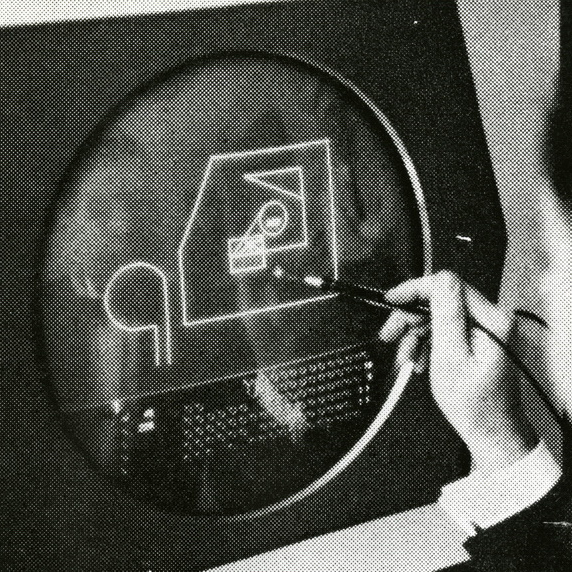
\includegraphics[width=8cm]{figuras/figura-1}}
		}{
			\Fonte{http://i0.wp.com/www.designleap.org/wp-content/uploads/2014/06/Sketchpad-Ivan-Sutherland-1963.jpg?resize=572\%2C572}
		}	
	\end{figure}
	\nocite{figura1}
	
Com o avanço resultado da criação dos circuitos integrados, cujo uso nos microprocessadores proporcionou um espantoso crescimento da indústria, os computadores deixaram de ser um monopólio das grandes companhias e tornaram-se muito mais acessíveis a pessoas simples. Isso abriu várias possibilidades para o mercado de computadores pessoais, entre elas destaca-se o surgimento das primeiras placas gráficas produzidas pela IBM (\acrlong{IBM}).

% \begin{figure}[h!]
    \centering
    \Caption{\label{fig:exemplo-2} Placa gráfica denominada Color Graphics Adapter produzida nos anos 80 pela IBM.}	
    \UNIFORfig{}{
        \fbox{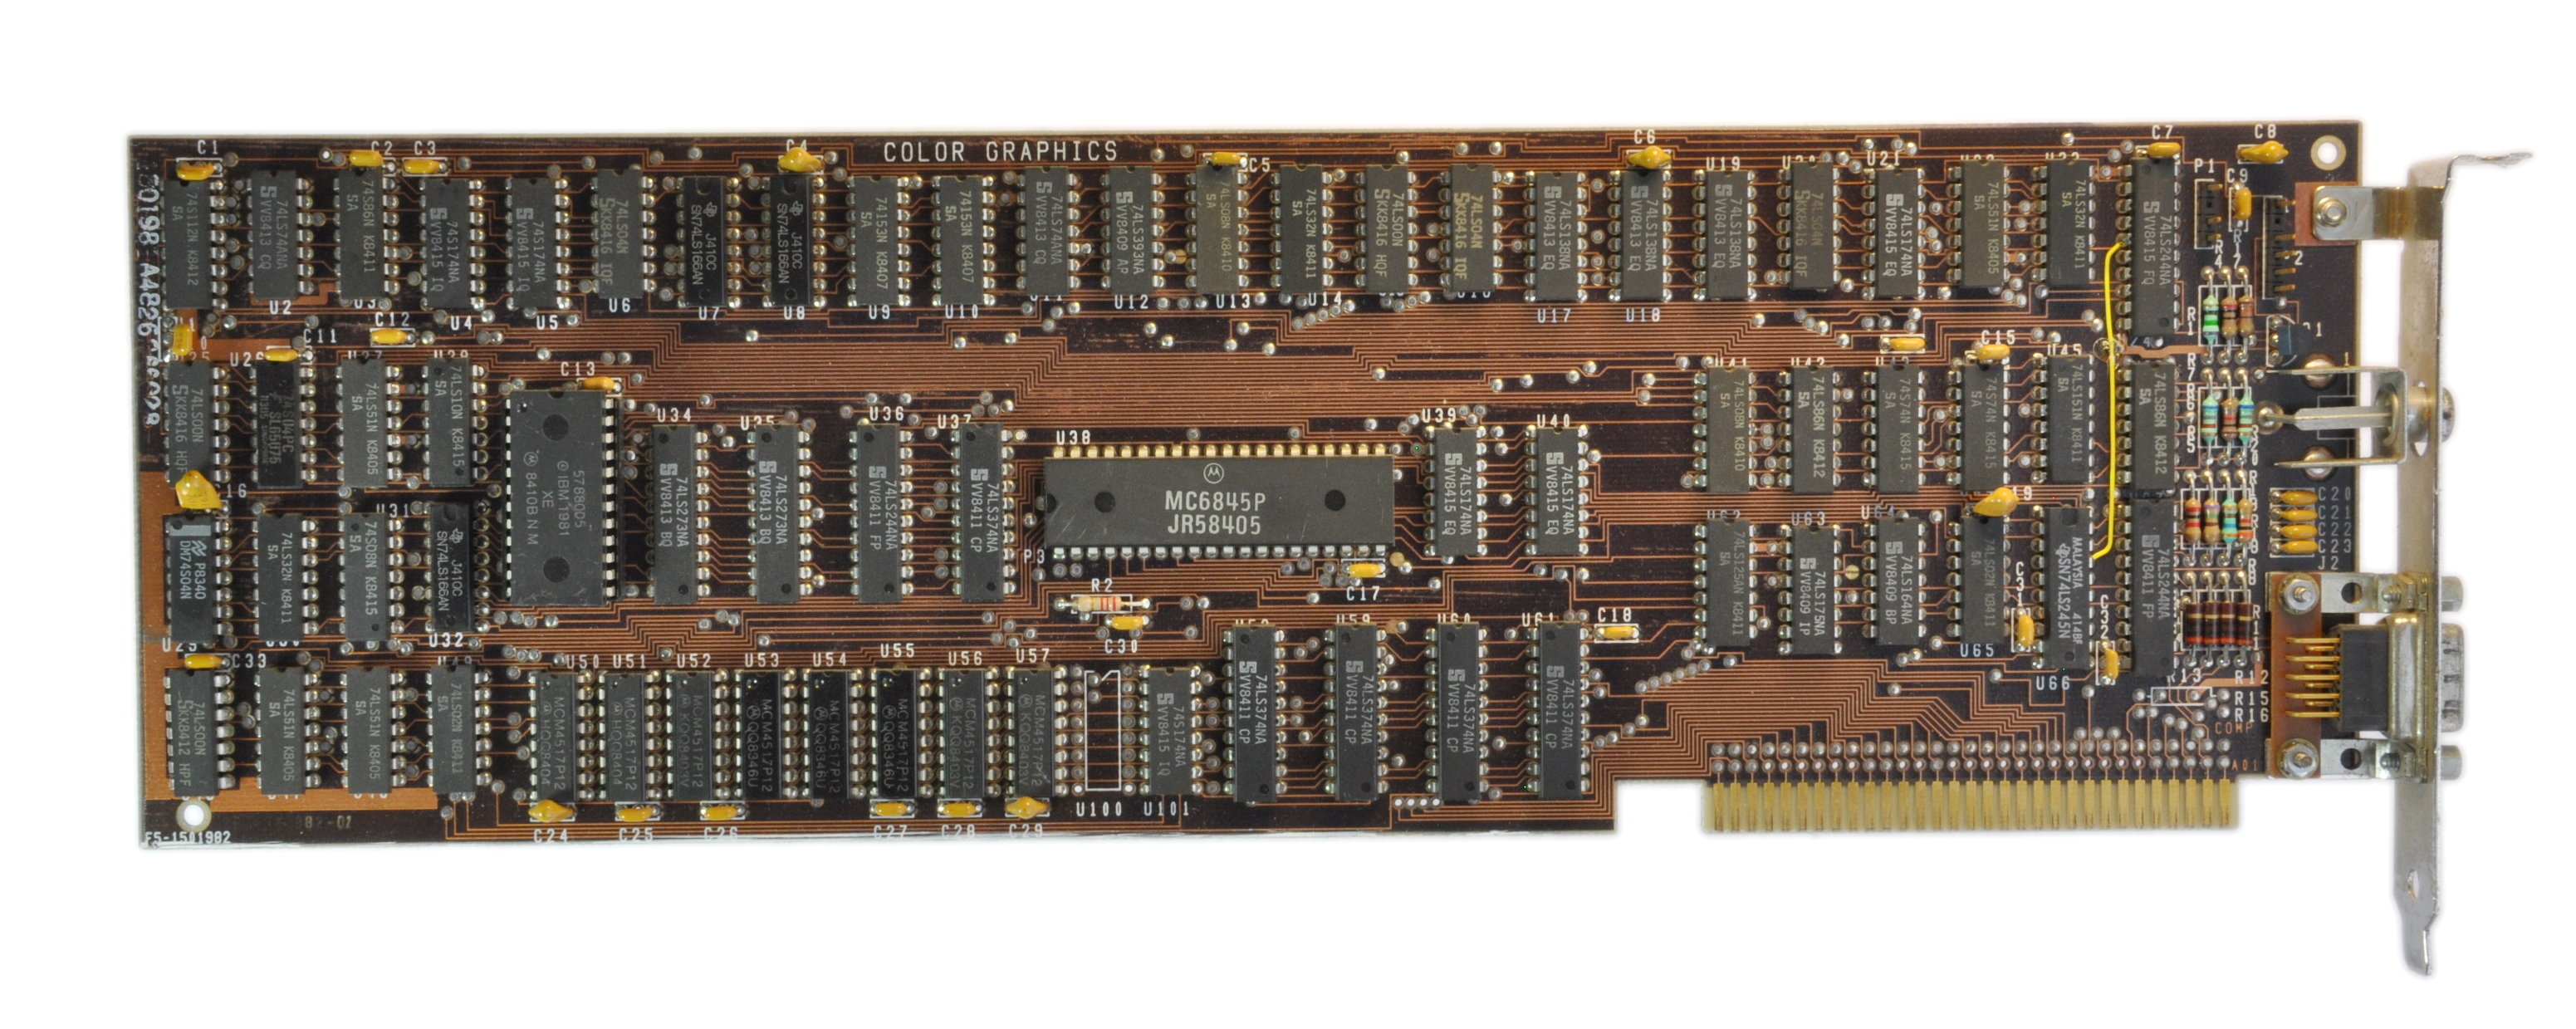
\includegraphics[width=15cm]{figuras/figura-2}}
    }{
        \Fonte{https://upload.wikimedia.org/wikipedia/commons/5/55/IBM\_Color\_Graphics\_Adapter.jpg}
    }	
\end{figure}
\nocite{figura2}    
	
Como a indústria de jogos eletrônicos tinha mais recursos para explorar devido às melhorias de hardware disponíveis, vários jogos começaram a se destacar no mercado. Entre eles os mais marcantes para a popularização do uso de tecnologia de computação gráfica tridimensional foram lançados pela empresa id Software na década de 90. O primeiro sendo Wolfenstein 3D --- que na realidade utilizava o modo 7 do Super NES (\acrlong{NES}) para emular a ambientação tridimensional --- que definiu o padrão para jogos no gênero de tiro em primeira pessoa em 3D e o segundo sendo Doom que fazia uso de renderização com perspectiva 3D em tempo real por meio de software desenvolvido pela própria id Software voltado a produção para computadores que utilizavam o sistema operacional da Microsoft (\acrshort{MS-DOS}).

    \begin{figure}[h!]
		\centering
		\Caption{\label{fig:exemplo-3} No lado esquerdo percebe-se que Doom fazia uso de 3D real enquanto no lado direito Wolfenstein posicionava imagens 2D em diferentes camadas para simular a profundidade tridimensional.}	
		\UNIFORfig{}{
			\fbox{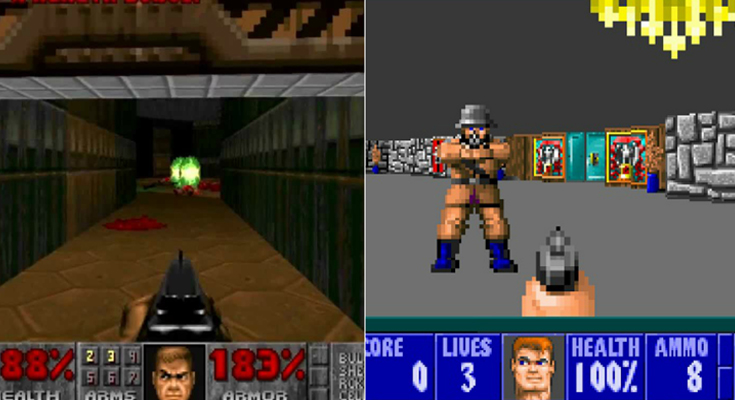
\includegraphics[width=13cm]{figuras/figura-3}}
		}{
			\Fonte{https://www.retrorefurbs.com/wolfenstein-vs-doom-the-battle-of-the-first-person-shooters/}
		}
	\end{figure}
	\nocite{figura3}

É de referir que a indústria de jogos eletrônicos apresenta incriveis taxas de crescimento e que desde 2017 conquista cada vez mais espaço no mercado. O valor do mercado de jogos atingiu a importante marca de US\$ 135 bilhões em 2018. Mas esse sucesso não é exclusivo de hoje, pois as empresas do ramo, desde a década de 70, apresentam crescimento constante e acelerado de suas receitas. Por isso cada vez mais empresas surgem dentro desse mercado a cada ano \cite{comparacaoDesempenho2}. 
	
Paralelo ao cenário desses jogos (LUTEN, 2014)\nocite{openGLBook}, a Silicon Graphics (\acrshort{SGI}), uma companhia especializada em computação gráfica 3D e líder de mercado na época, trabalhava no lançamento da Open Graphics Library (\acrshort{OpenGL}), uma API (\acrlong{API}) open source padronizada multiplataforma de processamento de gráficos de computador em tempo real que rapidamente dominou o mercado, e que era uma derivação de outra biblioteca proprietária da mesma empresa, a IRIS GL (\acrlong{IRIS GL}). 

Vendo uma oportunidade de mercado, a Microsoft logo agiu e comprou a empresa RenderMorphics, criadora da \acrshort{API} Reality Lab, que teve o nome alterado para Direct3D e foi distribuido como um SDK (\acrlong{SDK}) conhecido como DirectX (LUTEN, 2014)\nocite{openGLBook}, acabando por se tornar o concorrente direto da \acrshort{OpenGL}. Essa rivalidade no final das contas acabou sendo benéfica tanto para o mercado de jogos eletrônicos quanto para os seus consumidores, já que acelerou o desenvolvimento de novas tecnologias que exploravam ao máximo o potencial do hardware disponível.
	
 	\begin{figure}[h!]
		\centering
        \Caption{\label{fig:1} Hardware da placa gráfica da NVIDIA.}
        \begin{subfigure}{0.50\textwidth}
        \UNIFORfig{}{
			\fbox{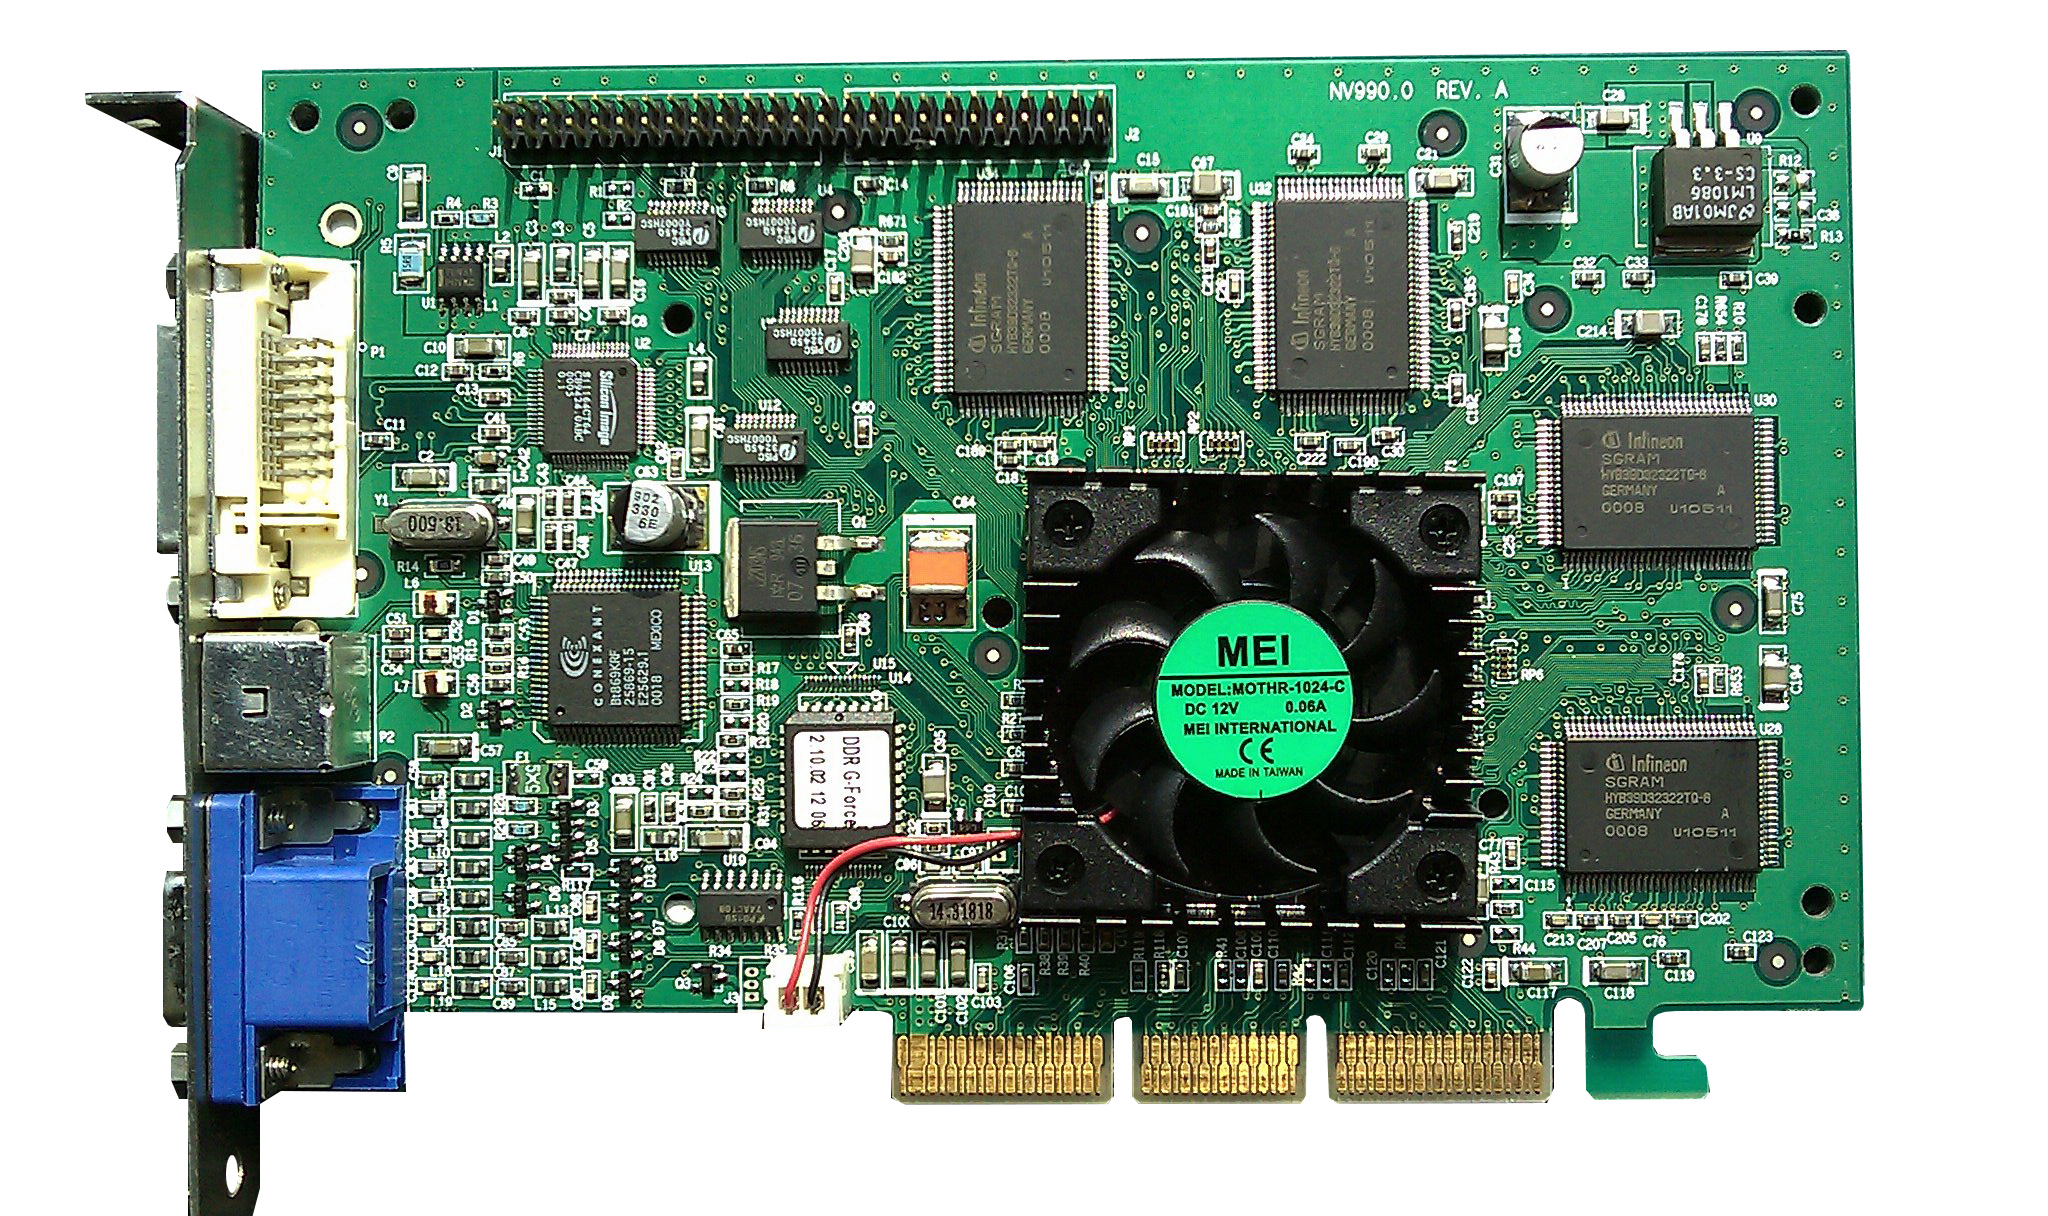
\includegraphics[width=\linewidth]{figuras/fig-a}}
		}{
		    \caption{GeForce 256} \label{fig:1a}
		}
		\nocite{figura4a}
        \end{subfigure}%
        
        \begin{subfigure}{0.30\textwidth}
        \UNIFORfig{}{
			\fbox{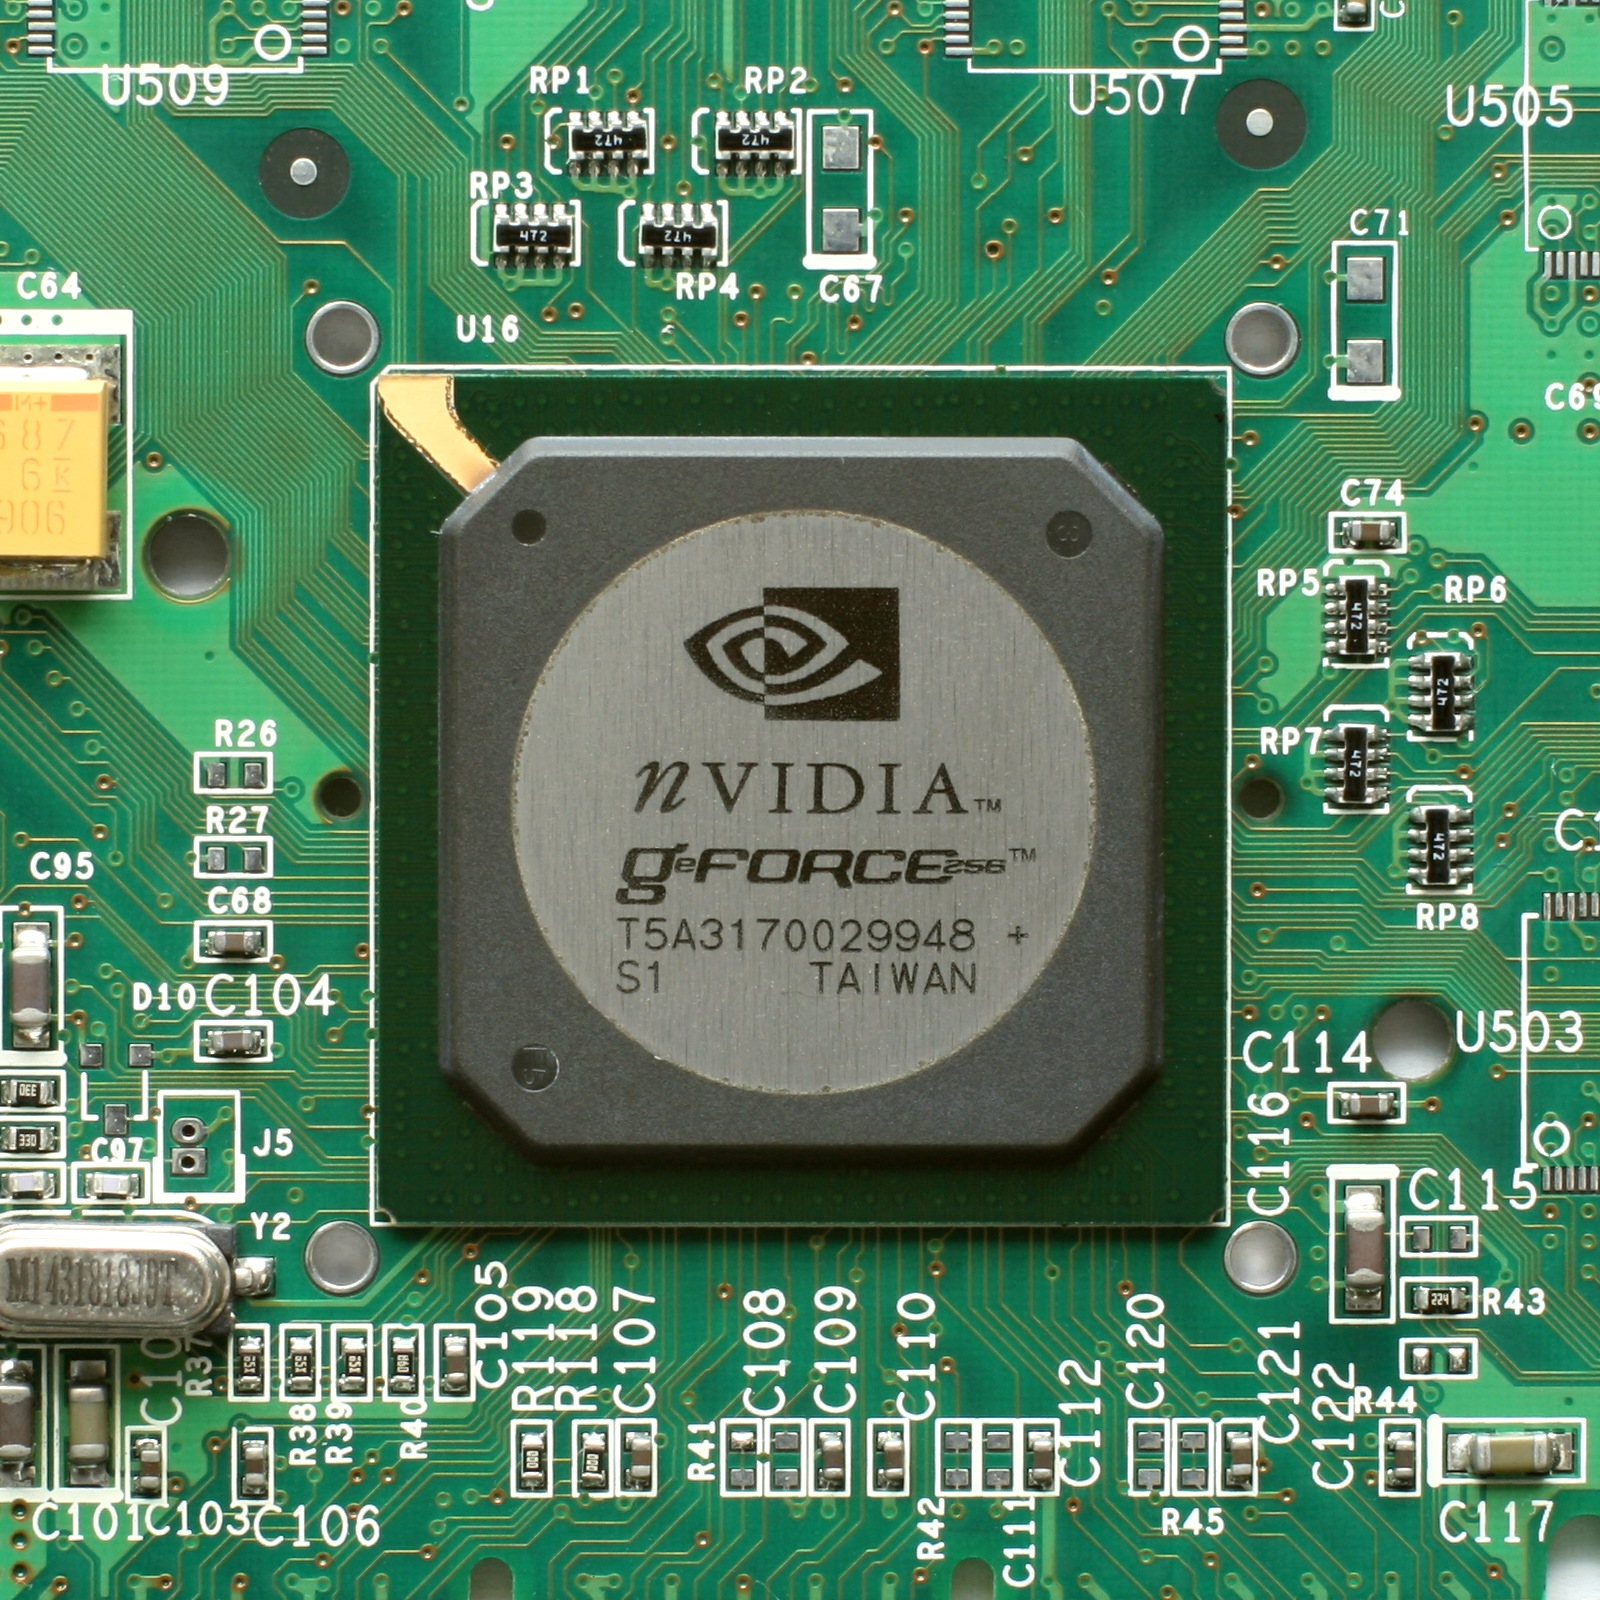
\includegraphics[width=\linewidth]{figuras/fig-b}}
		}{
		    \caption{GPU da GeForce 256} \label{fig:1b}
		}
		\nocite{figura4b}
        \end{subfigure}
		{
			\Fonte{https://upload.wikimedia.org/wikipedia/commons}
		}
	\end{figure}

Mais adiante, em 1999, a empresa NVIDIA foi responsável for trazer mais uma inovação ao mercado, a "primeira GPU" (\acrlong{GPU}) foi como ficou conhecida a placa gráfica GeForce 256 (Figura 4), que fazia uso de uma tecnologia chamada T\&L (\acrlong{T+L}) que basicamente movia os cálculos de transformação e iluminação de vértices da CPU (\acrlong{CPU}) para a \acrshort{GPU}. Isso permitia uma maior velocidade em operações matemáticas de ponto flutuante. Então nos próximos anos o que se viu foi um crescimento exponencial de performance de \acrshort{GPU} para renderização em tempo real.

Uma GPU é um circuito eletrônico projetado para realizar manipulaçoes rápidas em memória para acelerar a criação de imagens em um buffer de quadros que envia a saída para uma tela. Em aplicações que exigem muitas operações vetoriais, o poder de computação paralelo da GPU consegue entregar maior performance que uma CPU convencional. Daí seu vasto uso em jogos eletrônicos, mas também em outras áreas, principalmente na ciência \cite{shea2013gpu}.

Até então shaders eram bastante utilizados por melhorar a performance eliminando carga de trabalho excessiva da \acrshort{CPU}, porém sua programação era difícil devido a sintaxe utilizada ser semelhante à programação em Assembly. A Microsoft então lançou a versão 9.0 do Direct3D que trazia consigo a implementação da HLSL (\acrlong{HLSL}) que como o nome sugere permitia a programação de shaders em alto nível e possuia uma sintaxe bastante parecida com C. Enquanto isso, OpenGL também trouxe a sua própria linguagem de alto nível chamada GLSL (\acrlong{GLSL}) para competir no mercado (LUTEN, 2014)\nocite{openGLBook}. 

\subsection{Como o OpenGL funciona}
\label{sec:como-opengl-funciona}

Grosso modo, a API do OpenGL desenha gráficos em uma memória especializada em quadros de imagem (frame buffer) e os lê novamente quando precisa. O seu design único oferece suporte tanto a geometrias 3D quanto a imagens simples. O modelo de funcionamento dessa API pode ser descrito como cliente-servidor, pois a aplicação (cliente) faz solicitações por meio de comandos que são interpretados e processados pela implementação OpenGL (servidor) \cite{GLSLBook}. É importante destacar que a sincronia entre cliente e servidor e suas informações/dados não ocorre quando um comando é executado mas sim quando ele é emitido.

Os comandos são sempre processados na ordem em que são recebidos pelo servidor (execução fora de ordem não é permitida). Os dados passados para um comando OpenGL são então interpretados e copiados em memória caso seja necessário e as modificações subsequentes feitas pela aplicação não surtem efeito nos dados que estão armazenados internamente pelo OpenGL. Esses procedimentos são uma forma de garantir que um primitivo --- segundo Abdala (2019)\nocite{abdala}, uma representação discreta em grade de um elemento geométrico fundamental, e.g. ponto, linha, círculo, etc --- seja desenhado apenas se o primitivo anterior houver sido completamente desenhado \cite{GLSLBook}.

OpenGL foi projetada para atuar como uma máquina de estados composta de parametros que definem o comportamento da pipeline de renderização e da forma que as primitivas são transformadas em pixels na tela. O estado é composto por uma estrutura de dados chamada contexto gráfico que é gerenciada pelo sistema de janelas do SO (\acrlong{SO}) \cite{GLSLBook}. 

O principio básico de funcionamento dessa API é transformar dados vindos de uma aplicação em algo visível na tela, esse processo é chamado de renderização e normalmente é acelerado por um hardware com design específico chamado de acelerador gráfico, entretanto suas operações podem ser parcial ou totalmente implementadas por software executado pela CPU. Aceleradores gráficos tipicamente possuem região de memória delimitada para manutenção do conteúdo exibido na tela, sendo que cada pixel é representado por uma quantidade de bytes na memória; uma tela em escala de cinza, por exemplo, pode fazer uso de um byte para representar a tonalidade de cinza de cada pixel \cite{GLSLBook}.

Essa região conhecida como memória de exibição é escaneada "x" vezes por segundo para eliminar a cintilação. Há ainda uma região específica para manipular dados que não são visíveis na tela chamada de memoria de não exibição. O responsável pela alocação de memória é o próprio sistema operacional que suporta o OpenGL. Em um sistema de janelas, a janela que corresponde a região da memória gráfica que é modificada durante a renderização é chamada de frame buffer. Já em um cenário sem janelas (i.e. tela cheia) o frame buffer corresponde a toda a tela \cite{GLSLBook}.

\begin{figure}[h!]
	\centering
	\Caption{\label{fig:exemplo-6} O buffer de profundidade é mostrado em tons de cinza sendo que objetos próximos ficam com tonalidade mais escura enquanto objetos distantes assumem uma tonalidade mais clara.}	
	\UNIFORfig{}{
		\fbox{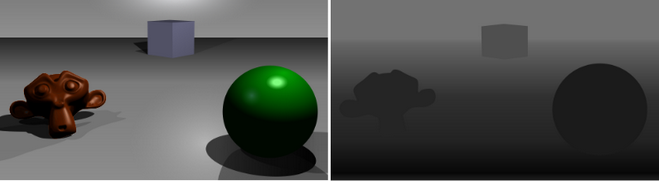
\includegraphics[width=15cm]{figuras/figura-6}}
	}{
		\Fonte{https://larranaga.github.io/Blog/imagenes/z-buffer.png}
	}
\end{figure}
\nocite{dptbuf}

Para que uma janela consiga suportar a renderização ela precisa de uma combinação de alguns elementos: até quatro buffers para as cores, um buffer de profundidade (Figura 5), um \textit{stencil buffer} (Figura 6), um buffer de acumulação, um \textit{multisample buffer} e um ou mais buffers auxiliares. A maioria dos hardwares suporta o carregamento duplo, técnica que faz uso de um buffer frontal e um buffer posterior para que o processo de renderização seja realizado em plano de fundo e então quando terminar seu conteúdo é trocado com o do buffer frontal para exibir o resultado final e iniciar a nova renderização. Isso ajuda a conseguir animações suaves à taxas interativas \cite{GLSLBook}.

\begin{figure}[h!]
	\centering
	\Caption{\label{fig:exemplo-7} O stencil buffer permite a customização da forma como objetos 3D são renderizados.}	
	\UNIFORfig{}{
		\fbox{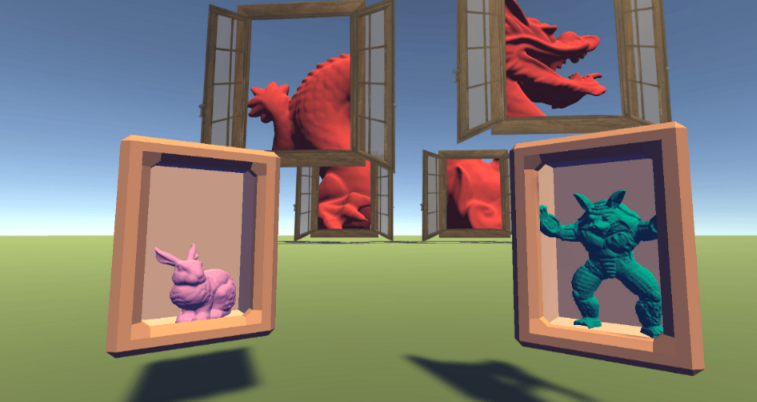
\includegraphics[width=15cm]{figuras/figura-7}}
	}{
		\Fonte{https://www.ronja-tutorials.com/assets/images/posts/022/Result.gif}
	}
\end{figure}
\nocite{stcbuf}
	
No caso do suporte a visualização 3D estéreo, mais dois buffers serão utilizados em conjunto com os dois citados anteriormente para criar uma combinação com quatro buffers de cor que são divididos para cada olho. Se um objeto 3D precisa ser desenhado com remoção de superfície encoberta, o buffer de profundidade entra em ação comparando o valor da profundidade de cada pixel dos objetos em cena para determinar qual será visível ou obscurecido. E há ainda a opção do uso de um \textit{stencil buffer} para aplicar operações complexas utilizando máscaras com o objetivo de determinar onde cada pixel deve ser atualizado ou não \cite{GLSLBook}.

O buffer de acumulação é capaz de reproduzir efeitos complexos como suavização em tela cheia de alta qualidade, profundidade de campo e desfoque de movimento. Ele funciona como um buffer de cor, porém com maior precisão, capaz de acumular imagens para produzir uma úncia imagem composta. Seguindo essa linha, o \textit{multisample buffer} é capaz de produzir várias amostras da renderização para realizar suavização sem precisar renderizar a cena mais de uma vez \cite{GLSLBook}. Por último, os buffers auxiliares servem para guardar dados genéricos. 

\subsubsection{Pipeline gráfica do OpenGL}
\label{sec:pipeline-opengl}

Para que a máquina de estados do OpenGL possa operar corretamente, foi definida uma ordem específica em que as operações envolvidas no processo de renderização precisam ser realizadas, essa padronização é chamada de \textit{pipeline} gráfica \cite{GLSLBook} e pode ser vista na Figura 7. Todos os dados necessários para desenhar a geometria estão contidos em espaço em memória e podem ser lidos pelo OpenGL de três maneiras diferentes. 

\begin{figure}[h!]
	\centering
	\Caption{\label{fig:pipeline} Pipeline gráfico do OpenGL.}	
	\UNIFORfig{}{
		\fbox{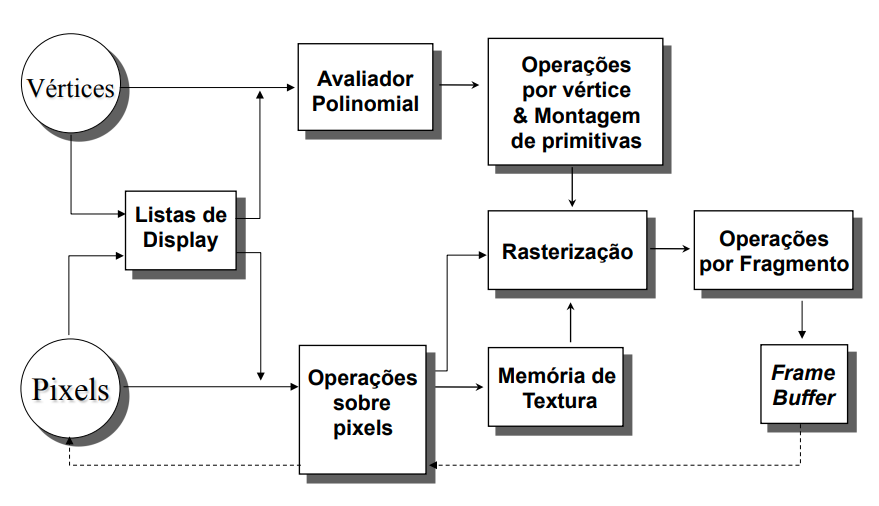
\includegraphics[width=13cm]{figuras/pipeline.png}}
	}{
		\Fonte{\url{http://www.ic.uff.br/~anselmo/cursos/CGI/slidesGrad/CG_aula4(introducaoaOpenGL).pdf}}
	}
\end{figure}
\nocite{pipeline}

A primeira seria enviar um vértice de cada vez utilizando alguns comandos intermitentes para manipular atributos dos vértices. A segunda seria utilizar matrizes de vértices, o que oferece melhor performance devido a forma de organização dos dados, pois são utilizados ponteiros e mais dados podem ser processados de uma vez. Esses dois casos citados acima fazem uso do modo imediato pois as primitivas são renderizadas assim que são especificadas \cite{GLSLBook}. 

O terceiro modo seria utilizar algum dos dois procedimentos citados acima implementando uma lista de exibição, que é uma estrutura de dados que guarda comandos para execução futura. Algumas vantagens desse método no que diz respeito a performance seria a possibilidade de otimizar os comandos contidos na lista, ou ainda guardar os comandos na memória do acelerador gráfico para uma melhor performance de desenho \cite{GLSLBook}. 
	
Como todas as primitivas geométricas podem ser descritas por vértices, as curvas e as superfícies podem ser descritas pelas funções polinomiais chamadas funções base. A função do avaliador polinomial nesse caso é derivar os vértices para conseguir representar superfícies e curvas. Isso é feito através do método de mapeamento polinomial, que produz as normais da superfície, as coordenadas da textura, as cores, e valores de coordenadas espaciais dos pontos de controle (VIEIRA, 2017)\nocite{pipelnRef}.

A próxima etapa é o estágio das operações por vértice que converte os vértices em primitivas. Alguns dados do vértice são transformados em matrizes de pontos flutuantes. Nesta etapa ocorre a projeção de coordenadas do espaço do mundo para o espaço da tela. Inclui algumas etapas como geração e transformação de coordenadas de textura, e também cálculos de luz para produção dos valores de cor (VIEIRA, 2017). Por isso é normal que essa etapa exija mais recursos computacionais. 

Logo em seguida ocorre a montagem das primitivas por meio do \textit{clipping} (eliminação de parte da geometria desnecessária para a renderização), que é um processo onde se a primitiva está totalmente dentro do plano de visualização ela é repassada para o devido processamento. Caso ela esteja totalmente fora do plano de visualização ela é rejeitada e não é processada. Se a primitiva estiver parcialmente visível no plano, ela é dividida para que somente a porção visível siga para processamento.

Outra operação que ocorre nesse estágio é a projeção das coordenadas da perspectiva para coordenadas da janela. Além disso, há ainda uma etapa opcional de \textit{culling} onde os polígonos são testados para saber se será preciso descartar faces posteriores, anteriores ou ambas \cite{GLSLBook}. Paralelamente a esse processo, os dados de pixels contidos em uma matriz na memória do sistema são empacotados e escalados, inclinados e processados por um mapa de pixels. Os resultados, que serão então empacotados em um formato apropriado e retornados a uma matriz de memória do sistema, podem ser escritos na memória da textura ou emitidos à uma etapa de rasterização.

Rasterização é a etapa de conversão de dados tanto geométricos como de pixel em fragmentos. Cada fragmento passa por mais algumas operações como: \textit{texturing}, onde um elemento da textura é gerado e aplicado da memória da textura para cada fragmento; aplicação do valor de cor e profundidade; cálculos de névoa; testes de profundidade, transparência e remoção de faces ocultas (VIEIRA, 2017). Ao final são armazenados os valores no \textit{frame buffer}. Apesar de possuir muitos processos, é uma etapa relativamente simples e pode ser executada eficientemente para milhões de pixels por segundo com o hardware disponível atualmente.

Sobre a etapa de texturização é interessante destacar que a API tem capacidade de trabalhar com quatro tipos de texturas. Texturas de uma dimensão (vetor de pixels), texturas 2D (matriz $ mxn $ de pixels), texturas 3D (matriz com uma dimensão a mais para guardar informações adicionais e.g. profundidade), e mapas cúbicos (normalmente usado para simular reflexões de ambiente). A API também pode trabalhar com formatos de imagem compactados, esses usam significativamente menos memória e melhoram a performance \cite{GLSLBook}.

É importante destacar que a API também fornece a possibilidade de utilizar texturas do tipo \textit{mipmap} --- várias representações da mesma imagem, porém cada uma tem metade da resolução da anterior --- em conjunto com o parâmetro de nível de detalhe que será detalhado mais adiante, mas que de forma simplificada permite a otimização do processo de renderização de objetos que estão distantes da câmera. 

\begin{equation} \label{eq-pipeline}
	\begin{aligned}
		f((x,y), \mathbf{v})=p \circ r(g \circ h(\mathbf{v}), (x,y)) 
	\end{aligned}
\end{equation}

Uma descrição matemática da pipeline de renderização está na Equação \ref{eq-pipeline} onde (x, y) é a posição na tela de cada pixel, \textbf{v} é um conjunto de primitivas, p é o shader de fragmentos, g é o shader de geometria, h é o shader de vértice e r é o estágio de rasterização onde as primitivas são convertidas em pixels com atributos de geometria interpolados \cite{wang2014auto}.

Por fim, é importante mencionar que existem dois modos principais de renderização: o modo direto calcula as luzes e materiais para cada geometria visível e depois resolve qual está mais próxima da câmera para então decidir quais exibir. Já o modo diferido realiza várias passadas (profundidade, cor, normais) para as geometrias e só então realiza os cálculos, dessa forma apenas os fragmentos visíveis são considerados. O segundo modo é mais eficiente para lidar com muitas luzes, porém não oferece suporte a transparência e suavização \cite{vsmid2017comparison}.

\subsubsection{Matrizes de transformação de coordenadas}
\label{sec:matrizes-transformacao-coordenadas}

\begin{figure}[htp]
	\centering
	\Caption{\label{fig:spaces} Processo de transformação entre os sistemas de coordenadas e seus espaços.}	
	\UNIFORfig{}{
		\fbox{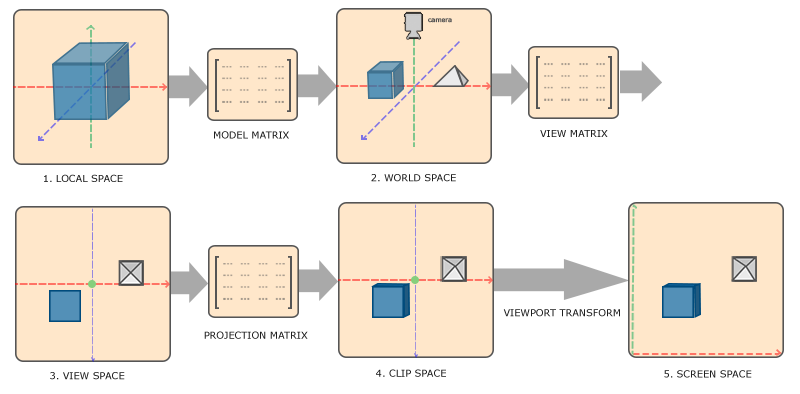
\includegraphics[width=12cm]{figuras/spaces.png}}
	}{
		\Fonte{\url{https://learnopengl.com/img/getting-started/coordinate_systems.png}}
	}
\end{figure}
\nocite{spaces}

Esse é um tópico mais complexo, mas que também é importante para entender como a pipeline gráfica do OpenGL transforma descrições de objetos tridimensionais em imagens 2D que são exibidas na tela (Figura \ref{fig:spaces}). Algo semelhante a como uma câmera pode ser usada para criar uma representação em imagem de algo no mundo real. Entretanto nesse caso o primeiro passo consiste em pegar as informações do modelo do objeto 3D, como posição dos vértices e normais da superfície, para interpretá-las como coordenadas do espaço do objeto \cite{GLSLBook}. 

Como cada objeto tem suas próprias características é necessário definir um sistema de coordenadas uniforme para que seja possível usar vários objetos em uma única cena. Para isso é utilizado o sistema de coordenadas global, e aqui a API vai um passo além e realiza mais uma conversão para o sistema de coordenadas de olho levando em consideração a posição da câmera na cena, seu ponto focal (para onde a câmera está olhando) e o vetor de direção para cima (e.g. a orientação da câmera) \cite{GLSLBook}. 

	\begin{equation}
		\begin{bmatrix}
			x_{olho} \\
			y_{olho} \\
			z_{olho} \\
			w_{olho} \\
		\end{bmatrix}
		=
		M_{modelView} \cdot
		\begin{bmatrix}
			x_{obj} \\
			y_{obj} \\
			z_{obj} \\
			w_{obj} \\
		\end{bmatrix}
	\end{equation}

	\begin{figure}[h!]
		\centering
		\Caption{\label{fig:worldview} Conteúdo das quatro colunas da matriz \textit{modelView}.}	
		\UNIFORfig{}{
			\fbox{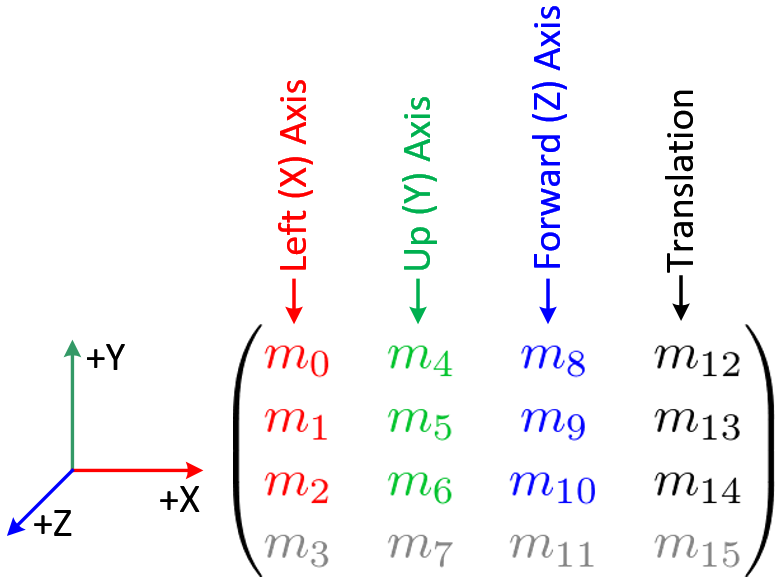
\includegraphics[width=6cm]{figuras/modelView.png}}
		}{
			\Fonte{\url{http://www.songho.ca/opengl/gl_transform.html}}
		}
	\end{figure}

Na equação 2.1, a matriz \textit{modelView} é uma multiplicação das matrizes de conversão de coordenadas de espaço de objeto para espaço global e de espaço global para espaço de olho. O cálculo das normais é semelhante, a diferença é que é utilizada a matriz transposta da inversa da matriz \textit{modelView} para multiplicar um vetor de normais. Como é possível ver na Figura \ref{fig:worldview} os três elementos mais à direita ($ m_{12} $, $ m_{13} $, $ m_{14} $) são para transformação de translação. O $ m_{15} $ é uma coordenada homogênea (Apêndice --- A) usada para transformação para o espaço de projeção. Os três conjunto de elementos ($ m_{0} $, $ m_{1} $, $ m_{2} $), ($ m_{4} $, $ m_{5} $, $ m_{6} $) e ($ m_{8} $, $ m_{9} $, $ m_{10} $) são usados para rotação e escala e representam os três eixos ortogonais x, y e z (AHN, 2013)\nocite{openglOnline}.

Após essa conversão, as coordenadas obtidas são multiplicadas pela matriz de projeção para definir como os vértices serão projetados na tela, os valores dessa matriz dependem se modo de projeção utilizado é em perspectiva ou ortográfico (Figura \ref{fig:frustum}) e são mostrados nas equações \ref{eq-persp} e \ref{eq-ortho} respectivamente. 

	\begin{equation} \label{eq-persp}
		\resizebox{.35\hsize}{!}{$ M_{persp}
		=
		\begin{bmatrix}
			\cfrac{2n}{r-l} & 0 & \cfrac{r+l}{r-l} & 0 \\
			0 & \cfrac{2n}{t-b} & \cfrac{t+b}{t-b} & 0 \\
			0 & 0 & \cfrac{-(f+n)}{f-n} & \cfrac{-2fn}{f-n}\\
			0 & 0 & -1 & 0 \\
		\end{bmatrix} $}
	\end{equation}
	\begin{equation} \label{eq-ortho}
		\resizebox{.35\hsize}{!}{$ M_{orto}
		=
		\begin{bmatrix}
			\cfrac{2}{r-l} & 0 & 0 & -\cfrac{r+l}{r-l} \\
			0 & \cfrac{2}{t-b} & 0 & -\cfrac{t+b}{t-b} \\
			0 & 0 & \cfrac{-2}{f-n} & -\cfrac{f+n}{f-n}\\
			0 & 0 & 0 & 1 \\
		\end{bmatrix} $}
	\end{equation}

Os valores obtidos nessa operação são normalizados em uma região cúbica definida pelos pontos (-1, -1, -1) e (1, 1, 1) para espaço de coordenadas de dispositivo normalizado, isso significa que os valores passam a ser algum valor entre -1 e 1. Essa etapa é necessária para qua a área de visualização seja apropriadamente mapeada em uma janela de exibição de tamanho arbitrário. Por último, as coordenadas são convertidas para o sistema de coordenadas de tela. A partir desse ponto elas continuam para o processo de rasterização da pipeline do OpenGL (AHN, 2013)\nocite{openglOnline}. 
	\begin{figure}[h!]
		\centering
        \Caption{\label{fig:frustum} Modos de projeção de câmera. As letras correspondem a \textit{left, right, bottom, top, near e far}.}
        \begin{subfigure}{0.45\textwidth}
        \UNIFORfig{}{
			\fbox{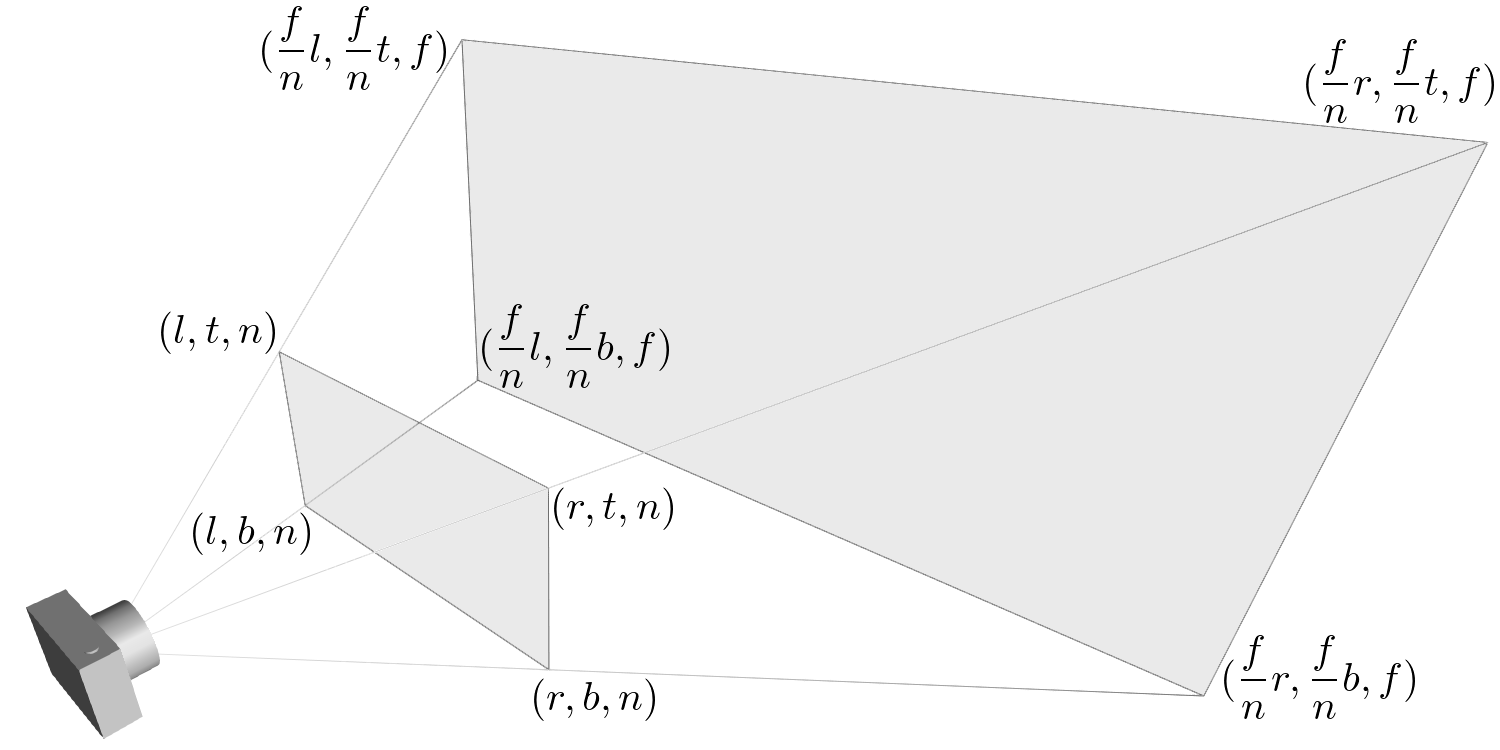
\includegraphics[width=\linewidth]{figuras/persp.png}}
		}{
		    \caption{\Gls{view-frustum} em perspectiva}
		}
        \end{subfigure}
		\hfill
        \begin{subfigure}{0.47\textwidth}
        \UNIFORfig{}{
			\fbox{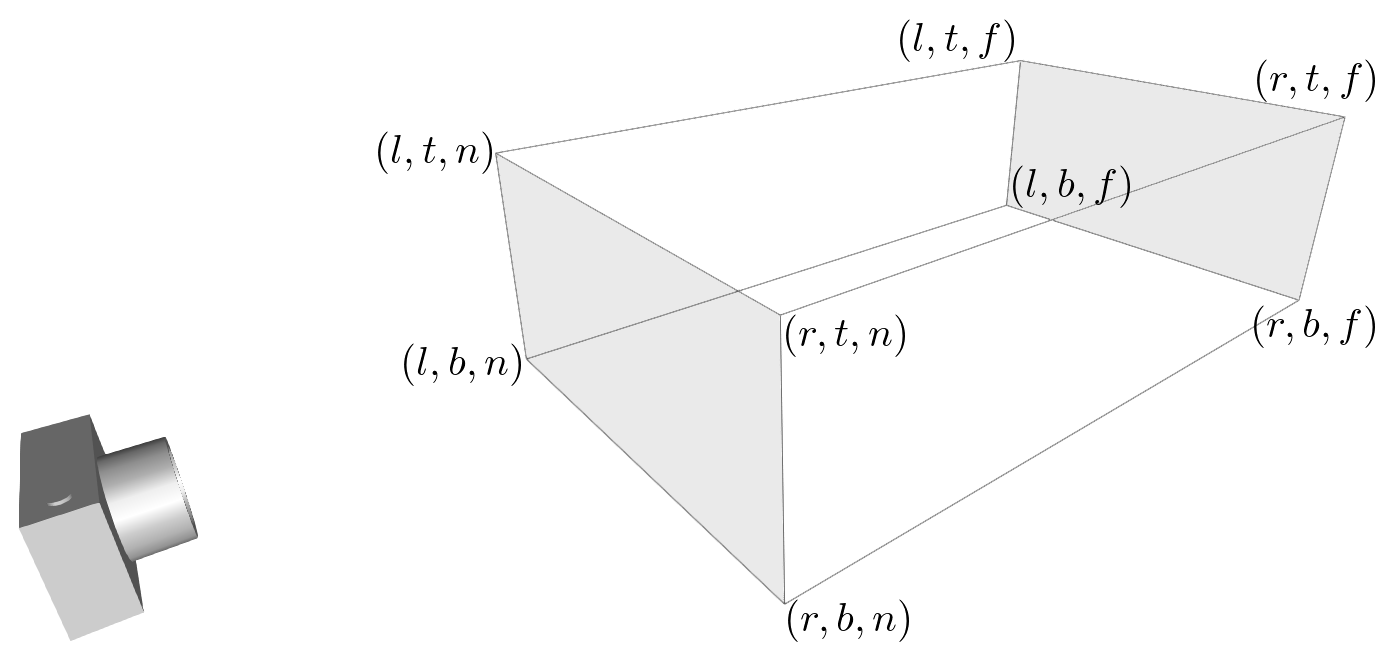
\includegraphics[width=\linewidth]{figuras/ortho.png}}
		}{
		    \caption{\Gls{view-frustum} ortográfico}
		}
        \end{subfigure}
		{
			\Fonte{\url{http://www.songho.ca/opengl/gl_transform.html}}
		}
	\end{figure}

\subsection{OpenGL Shading Language}
\label{sec:glsl}

Devido à necessidade crescente de substituir funcionalidades fixas por programabilidade em áreas que ficavam cada vez mais complexas, como processamento de vértices e fragmentos, foi desenvolvida uma solução que adicionou estágios programáveis para resolver esse problema. Essa solução foi a introdução da linguagem de sombreamento \acrshort{GLSL}, feita para ser executada nos dois processadores programáveis existentes no OpenGL: o processador de vértices e o processador de fragmentos (portanto os respectivos nomes \textit{vertex shader} e \textit{fragment shader}) \cite{GLSLBook}. 

Um shader pode então ser definido como um código escrito em uma linguagem de sombreamento (HLSL, GLSL, RSL e etc) com o propósito de ser executado por um dos processadores programáveis do OpenGL. Um programa de shader é então um conjunto de shaders compilados executáveis \cite{GLSLBook}. A Figura \ref{fig:outline} mostra a implementação do código-fonte \ref{cf:outline} para criar um efeito de linha de contorno em volta de um objeto 3D utilizando a linguagem GLSL.

\begin{figure}[h!]
	\centering
	\Caption{\label{fig:outline} Demonstração de um shader simples de linha contorno.}	
	\UNIFORfig{}{
		\fbox{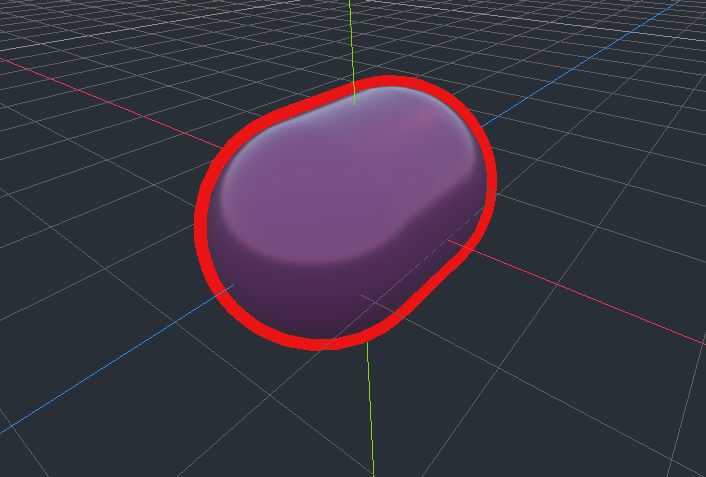
\includegraphics[width=8cm]{figuras/outline.png}}
	}{
		\Fonte{Elaborado pelo autor}
	}
\end{figure}

A linguagem de sombreamento GLSL faz uso de uma sintaxe bastante similar a linguagem de programação C. Seus tipos incluem vetores e matrizes por serem estruturas fundamentais para cálculos matemáticos com operações para gráficos 3D. O uso de números de ponto flutuante (\textit{float}) também é fundamental para conseguir altos níveis de precisão a troco de performance, por isso é possível especificar o nível de precisão desejado ao utilizá-los. Além disso ela oferece suporte a laços, chamadas a sub-rotinas, expressões condicionais e conta com funções embutidas próprias para o desenvolvimento de shaders \cite{GLSLBook}. 

Essa linguagem possibilitou aos desenvolvedores implementar um conjunto de diferentes técnicas para conseguir obter uma variedade enorme de efeitos visuais; não somente isso mas o fato de que essas técnicas são implementadas com aceleração via hardware pela GPU (com processamento paralelo) proporciona um aumento drástico de performance e libera carga da CPU para realizar outras tarefas \cite{GLSLBook}.

O processador de vértices é uma unidade programável que realiza operações nos valores de vértices recebidos e seus dados associados. Essas operações consistem em transformação de vértices, transformação e normalização das normais, geração e transformação das coordenadas de textura, iluminação e aplicação de cor. Shaders feitos para rodar nesse processador são chamados de shaders de vértice \cite{GLSLBook}. 

Variáveis de atributo (variável global somente leitura alterada por vértice) são utilizadas para passar valores da aplicação para o processador de vértices. Já as variáveis uniformes (variável global somente leitura alterada por primitiva) são utilizadas para passar dados tanto para o processador de vértices como de fragmentos. Por último há as variáveis variantes cuja função é transportar informação do processador de vértices para o processador de fragmentos \cite{GLSLBook}.

O processador de vértices atua em um vértice por vez e uma implementação pode ter múltiplos processadores operando em paralelo (o mesmo vale para o processador de fragmentos). Logo, o shader de vértice é executado uma vez para cada vértice, sendo que há uma possibilidade de perda de performance caso um shader de vértice precise calcular mais variáveis variantes do que o que é necessário pelo shader de fragmentos. Por outro lado, o processador de fragmentos é responsável por realizar algumas operações como interpolação de valores, acesso e aplicação de texturas, névoa e soma de cor \cite{GLSLBook}. 

Cabe ressaltar que, em termos de performance, normalmente os desenvolvedores preferem utilizar um shader de vértice mais genérico em conjunto com um shader de fragmento, pois assim é possível utilizar apenas um subconjunto das variáveis contidas no shader de vértice e ainda sim reduzir tempo e custos de desenvolvimento e manutenção para uma grande quantidade de shaders \cite{GLSLBook}.

\subsection{Direct3D (HLSL) \textit{versus} OpenGL (GLSL)}
\label{sec:direct-versus-opengl}

Direct3D é uma API para desenvolvimento de aplicações gráficas nativas para plataformas proprietárias da Microsoft. Ela evoluiu muito durante os anos anos 90 e superou a OpenGL. Conceitualmente, a pipeline gráfica de ambas APIs são bem semelhantes, mas uma diferença importante se dá em termos de design de gerenciamento dos estágios de shaders, onde OpenGL faz uso de um objeto (programa de shader) que contém múltiplos shaders enquanto que Direct3D expõe um contexto de renderização diretamente para a criação de shaders. Quanto às linguagens (GLSL e HLSL), são muito parecidas e os desenvolvedores conseguem transcrever instruções facilmente de uma para a outra (MICROSOFT, 2020)\nocite{Direct3D}.

Considerando a pouca diferença em capacidade de renderização existente entre essas duas interfaces, a escolha sobre qual usar depende muito da plataforma alvo de desenvolvimento. Direct3D é específica para plataformas da Microsoft e é amplamente suportada por fornecedores de hardware gráfico, especialmente em computadores desktop. OpenGL é open source e possui bastante aceitação no espaço de desenvolvimento mobile, principalmente devido ao desenvolvimento da OpenGL ES --- uma subseção do OpenGL projetada especialmente para sistemas embarcados como smartphones e consoles portáteis \cite{HLSLBook}.

Uma das principais diferenças é o ambiente de execução. O compilador HLSL traduz o código para linguagem de máquina que é processada pelo driver do DirectX. Enquanto que no caso do OpenGL os fornecedores de hardware, por serem responsáveis pela implementação do compilador, possuem muito mais liberdade para realizar otimizações em shaders. Para mitigar essa diferença a Microsoft fornece uma solução (DirectX Effects Framework) para desenvolvedores elaborarem programas de shaders iguais para hardwares com menor e maior capacidade de processamento \cite{GLSLBook}.

\subsection{High-Level Shader Language}
\label{sec:hlsl}

\begin{figure}[h!]
	\centering
	\Caption{\label{fig:outlineHLSL} O mesmo resultado de contorno obtido com HLSL.}	
	\UNIFORfig{}{
		\fbox{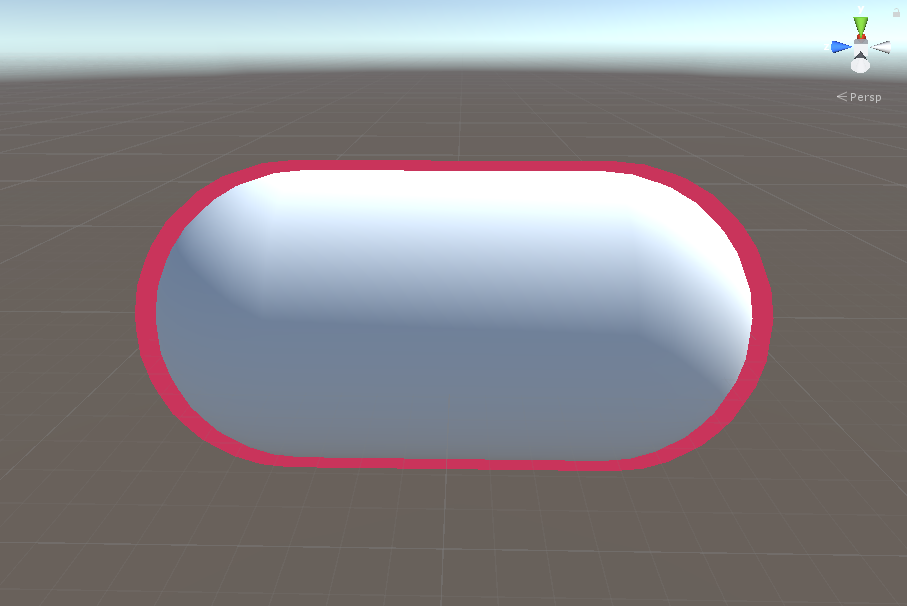
\includegraphics[width=7cm]{figuras/outlineUnity.PNG}}
	}{
		\Fonte{Elaborado pelo autor}
	}
\end{figure}

Essa é uma linguagem de shader criada em 2002 (acompanhou o DirectX 9) que também assemelha-se à linguagem C. Ao longo dos anos foram adicionadas melhorias como suporte a \textit{\Gls{multithread}}, adição de uma API para uso de GPGPU (\acrlong{GPGPU}) e suporte a tesselação. Na Figura \ref{fig:outlineHLSL} é mostrada a implementação de um shader de contorno (ver código-fonte \ref{cf:outlineHLSL}) similar ao anterior para realçar as diferenças e semelhanças entre as duas linguagens.

Uma GPU de propósito geral é uma unidade de processamento gráfico que realiza cálculos genéricos que normalmente seriam feitos pela CPU. São utilizadas para realizar tarefas custosas como cálculos de física, criptografia e computações científicas, pois é possível tirar proveito do paralelismo. Da mesma forma que um núcleo pode ser utilizado para renderizar múltiplos pixels simultaneamente, ele também é capaz de processar múltiplos fluxos de dados ao mesmo tempo (TECHTARGET, 2015)\nocite{GPGPU}.

Tesselação é mais um processo na pipeline gráfica responsável por adicionar detalhes a objetos diretamente pela GPU. De maneira geral, mais detalhes geometricos (mais vértices), resultam em uma renderização "mais bonita". Seu modo de funcionamento consiste em subdividir um objeto dinamicamente e sem o custo adicional de reprocessamento de geometria. Isso permite um sistema de nível de detalhe dinâmico e menos utilização do barramento de gráficos, o que melhora a performance \cite{HLSLBook}.

	\begin{figure}[h!]
		\centering
		\Caption{\label{fig:tess} Diferentes níveis de tesselação aplicados em uma malha produzem aumento no número de vértices.}	
		\UNIFORfig{}{
			\fbox{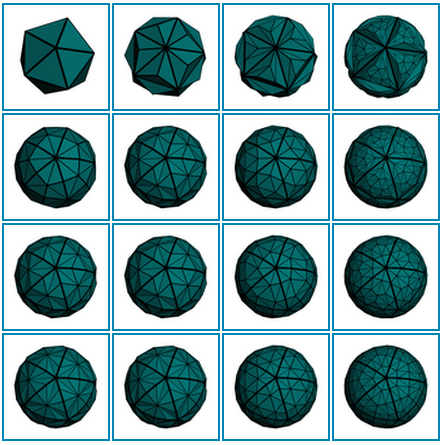
\includegraphics[width=8cm]{figuras/tess.png}}
		}{
			\Fonte{\url{https://upload.wikimedia.org/wikipedia/commons/f/fc/Tessellation_Level_Table.png}}
		}
	\end{figure}
	\nocite{tesselation}

Esse processo é relativamente novo e ocorre na etapa do shader de geometria, que adiciona um passo de criação de geometria na pipeline gráfica após o shader de vértices. Isso permite que o programador implemente tesselação automática para geometrias complexas, ou realize operações gráficas dependentes de geometria como silhuetas e sombras \cite{bailey2007}.

Nível de detalhe é um fator chave de otimização utilizado por game engines para alcançar renderização de alta qualiadade com melhor performance. Além disso é desejável evitar mudanças frequentes em shaders e chamadas de desenho utilizando um número reduzido de shaders. Isso minimiza a sobrecarga da CPU e ajuda a GPU a desenhar mais objetos em um frame com shaders com nível de detalhe \cite{yong2015rapid}.

\section{Aprofundando Conceitos Técnicos de Shaders}
\label{sec:aprofundando-conceitos-tecnicos-shaders}

A introdução do HLSL trouxe uma linguagem semelhante a C com estruturas extrar para tratar vetores, matrizes e outros elementos relacionados a graficos. Com a melhoria da legíbilidade e da produtividade, o seu uso permite aos desenvolvedores focar no código e reutilizar otimizações de alto nível (como fazer uso de tipos correspondentes e funções embutidas). O compilador HLSL contém truques de otimização de baixo nível que podem ajudar \cite{riguer2002performance}.

Ao estudar computação gráfica a dúvida mais comum ao se deparar com certos termos utilizados é "o que é um shader". Essa palavra pode causar uma certa estranheza no início mas sua definição não é nenhum bicho de sete cabeças. Shaders são apenas pequenos programas (assim como um reprodutor de mídia ou uma calculadora de um computador) que são executados diretamente pela \acrshort{GPU} ao invés da \acrshort{CPU}. Isso permite a redução da carga de trabalho gráfico da \acrshort{CPU} pelo redirecionamento das tarefas para a \acrshort{GPU} que possui hardware especializado para isso (LUTEN, 2014)\nocite{openGLBook}.

Um shader é um procedimento que computa alguns aspectos visuais de um objeto, como cor e deslocamento de superfície, tonalidade e direção da luz e efeitos volumétricos. São utilizados para especificar tranformações de vértices e cores de pixels. Pode-se pensá-los como uma função $ f $ que recebe um conjunto de valores (como coordenadas de posição, normais e texturas) $ v_i $ e um conjunto de parâmetros $ u_i $ (informação de cores e luz) e retorna a cor $ C_{xy} $ de cada objeto em cada pixel $ xy $ da imagem final \cite{fabio2005user}. 

Shaders programáveis são uma das ferramentas mais impressionantes desenvolvidas para computação gráfica nos últimos anos. Através de seu uso, programadores ganharam flexibilidade para aplicar efeitos vértice-por-vértice e pixel-por-pixel com o processamento paralelo em gráficos interativos entre as mais diversas áreas como ciência, arte, engenharia, entre outras \cite{bailey2007}.

	\begin{figure}[h!]
		\centering
		\Caption{\label{fig:exemplo-5} Demonstração de como é possível criar visuais únicos utilizando shaders.}	
		\UNIFORfig{}{
			\fbox{
\includegraphics[width=9cm]{figuras/figura-5}}
		}{
			\Fonte{Adaptado de \url{https://www.youtube.com/watch?time_continue=2&v=F0CWzpYY68A&feature=emb_logo}}
		}
	\end{figure}
	\nocite{figura5}

Tecnicamente falando, um shader contém um conjunto de instruções que são executadas concorrentemente para cada pixel desenhado na tela. Essa forma de operação abre um leque de possibilidades, onde é possível por exemplo atribuir um comportamento para cada pixel baseado na sua posição na tela. Em uma comparação com programação procedural, ele funcionaria como uma função que recebe uma posição e retorna uma cor, sendo que após a compilação seu tempo de execução é extremamente rápido (VIVO; LOWE, 2015)\nocite{bookOfShaders}.

Uma metáfora para ajudar a compreender a dimensão da complexidade do processamento de um shader seria imaginá-lo como um bloco de várias tarefas que passa por uma linha de produção industrial. As tarefas podem ser pequenas ou grandes e consequentemente podem demandar mais processamento e energia. No caso da CPU cada trabalho seguinte teria que esperar o término do atual para começar (VIVO; LOWE, 2015)\nocite{bookOfShaders}. É interessante ressaltar que hoje em dia existe a tecnologia de multiprocessamento, onde os computadores normalmente possuem grupos de quatro processadores que atuam em conjunto para realizar as tarefas.

Considerando uma tela com resolução de 800x600, significa que 480.000 pixels precisam ser processados a cada frame sendo que normalmente é utilizada uma taxa de 30 frames por segundo (\acrshort{FPS}), então será necessário fazer 14.400.000 cálculos por segundo. Isso explica o fato de video games e outras aplicações gráficas exigirem muito mais poder de processamento que outros programas. Seu conteúdo gráfico implica em inúmeras operações por cada pixel, pois cada pixel na tela precisa ser computado, e também em perspectivas e geometrias de jogos 3D (VIVO; LOWE, 2015)\nocite{bookOfShaders}.  

Esse cenário pode ser suficiente para sobrecarregar um microprocessador comum e fica pior quando leva-se em consideração as tecnologias que fazem uso seja de taxa de FPS maior, seja de resoluções maiores como 2K, e acima. Para resolver esse problema utiliza-se processamento paralelo. A GPU possui vários pequenos microprocessadores que funcionam concorrentemente, além disso ela possui funções matemáticas específicas aceleradas via hardware para realizar operações matriciais e trigonométricas rapidamente (VIVO; LOWE, 2015)\nocite{bookOfShaders}.

A dificuldade relativa de programar shaders levou ao desenvolvimento de ferramentas visuais que auxiliam a criação desses programas através do uso nós funcionais conectados entre si que remetem a uma estrutura de árvore. Esse tipo de ferramenta está presente na Unreal Engine desde 2005. Ao mesmo tempo que possuem utilidade, é importante garantir que shaders gerados por tais ferramentas seja otimizados. Otimização é importantíssima para encorajar desenvolvedores a criar shaders maiores e mais complexos \cite{jensen2007shader}.

Conforme descrito em estudo por \citeauthoronline{wang2014auto} (2014) vários estudos sobre otimização de shaders já foram conduzidos, porém com efetividade apenas para para o estágio de fragmentos. De certa forma a qualidade dos shaders depende bastante da experiência dos programadores e pode ser um processo bem demorado para níveis de complixadade maiores. Normalmente a computação mais custosa ocorre no shader de fragmentos. 

\subsection{Vertex Shader}
\label{vertex-shader}

Um shader de vértice é um programa executado uma vez para cada vértice cujo é atribuído. As operações mais importante dessa etapa são as que envolvem cálculo de transformação e luzes. A aplicação desses shader permite uma paleta ilimitada de efeitos visuais renderizadas em tempo real. Dentre as principais aplicações merecem destaque o suporte a criação de animações realistas e a possibilidade de deformar superfícies para criar efeitos realistas de ondas (NVIDIA, 2019)\nocite{vertexShader}.

	\begin{figure}[h!]
		\centering
		\Caption{\label{fig:shaderStages} Como os estágios de shaders se relacionam.}	
		\UNIFORfig{}{
			\fbox{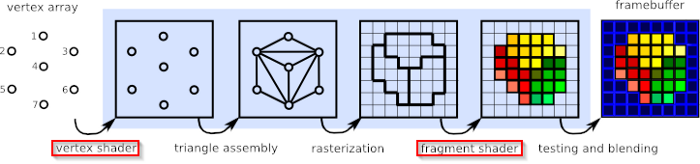
\includegraphics[width=13cm]{figuras/shaderStages}}
		}{
			\Fonte{\url{https://miro.medium.com/max/700/1*_z7Vbb0msvXsUFq3sSMZAg.png}}
		}
	\end{figure}
	\nocite{shaderStages}

O processador de vértices realiza as principais transformações de coordenadas descritas na Seção \ref{sec:matrizes-transformacao-coordenadas}. Como nessa etapa há bastante informação sobre a geometria e o processador é capaz de realizar inúmeras operações, essa é uma ótima etapa para inserir código. Quando essas coordenadas deixam o estágio de processamento, elas são cortadas e mapeadas para o sistema de coordenadas de tela, prontas para serem rasterizadas \cite{bailey2007}.

\subsection{Fragment Shader}
\label{sec:fragment-shader}

Um shader de fragmento é um programa executado uma vez para cada pixel. Fragmentos são estruturas de dados (contidas em cada pixel) que são criadas pela rasterização das primitivas. Um fragmento contém todos os dados necessários para atualizar seu espaço no \textit{frame buffer}. O processamento desses fragmentos consistem em operações feitas em cada pixel, sendo que as mais notáveis são a leitura da memória de textura e a aplicação do valor de textura para cada fragmento \cite{GLSLBook}. 

Nessa etapa o processador de fragmentos recebe as informações de cada pixel (seus valores de vermelho, verde, azul, transparência e coordenadas de textura). Cada pixel também possui informação recebida do processador de vértices e interpolada na rasterização. Esse processador também pode acessar informações globais como a posição das luzes e seu trabalho final é processar essas informações e produzir a cor final de cada pixel (ou descartá-lo). Sua grande utilidade consiste na possibilidade de customização da aparência dos pixels de acordo com as necessidades do programador \cite{bailey2007}. 

Dependendo da resolução definida, algo em torno de 2 milhões de pixels podem precisar ser processados e renderizados a cada frame (60 FPS). Isso facilmente gera uma carga computacional enorme. Felizmente, com a evolução da tecnologia, os desenvolvedores podem facilmente implementar programas que controlam a iluminação, o sombreamento e a cor de cada pixel (NVIDIA, 2019)\nocite{fragShader}.

Como foi mostrado por \citeauthoronline{bilodeau} (2019), apesar de ser possível realizar computações de propósito geral no shader de fragmentos, vale a pena destacar a tecnologia dos shaders de computação e suas vantagens como maior controle sobre as \textit{threads}, acesso à memória compartilhada, dispensabilidade de renderização de polígonos. Além disso, utilizar oclusão de ambiente em alta definição é muito custosa e pode ser substituida por meia resolução em conjunto com desfoque para melhorar a performance.

Shaders de fragmentos modernos são capazes de realizar centenas ou milhares de operações aritiméticas, incorporando funções trigonométricas custosas e vários acessos a mapas de textura para produzir a cor final de cada pixel. Consequentemente, seu custo de execução pode facilmente dominar a capacidade computacional por quadro \cite{lei2008acm}.

\section{Motores de jogo e suas ferramentas}
\label{sec:motores-jogo-ferramentas}

Um conjunto de ferramentas para criar um jogo é geralmente chamado de motor de jogo. Elas variam desde uma IDE (\acrlong{IDE}) até um pacote de software com capacidade de simulação física, renderização, rede e inteligência artificial. Podem ser classificadas pelas dificuldade de uso, plataformas de destino ou gênero de jogo que podem criar \cite{compGameLang}. 

Criadores de jogos atualmente contam com motores de jogo para desenvolver as principais partes de software para seus jogos. Sua principal função é simplificar as tarefas dos desenvolvedores oferecendo abstrações convenientes para os sistemas operacionais e seus hardwares nos quais o jogo funcionará. Isso somado ao propósito de explorar ao máximo a capacidade das máquinas dos usuários para que seja proporcionada uma experiência mais imersiva possível \cite{simon2015unity}.

\begin{quadro}[h!]	
	\centering
	\Caption{\label{qua:engines} Principais componentes das \textit{game} \textit{engines}}\UNIFORqua{}{
		\begin{tabular}{|l|c|m{3cm}|c|}
			\hline
			\phantom{engines} & Godot & \centering Unity & Unreal \\
			\hline
			Shading & GLSL & \centering ShaderLab (HLSL) / \textit{Shader} Graph & Material Nodes \\
			\hline
			Sistema de Partículas & Built-in & \centering Built-in / VFX Graph & UnrealCascade\\
			\hline
			Motor de física & Bullet & \centering PhysX  & PhysX \\
			\hline
			Programação & GDSCript / C\# & \centering C\# & C++ / BluePrint \\
			\hline
			Audio & Bus System & \centering Audio Mixer & Sound Cue \\		
			\hline
		\end{tabular}
	}{
		\Fonte{Elaborado pelo autor (2021)}
	}
\end{quadro}


Conforme definido por Barczak, Woźniak (2019) motores de jogo são softwares (proprietários ou de código aberto) voltados para facilitar a criação de jogos eletrônicos. Seus sistemas permitem a integração de vários elementos como \textit{\Gls{scripts}}, malhas, animações e audios que juntos podem formar um jogo eletrônico que pode ser distribuído para diferentes plataformas por indivíduos ou companhias. 

Atualmente motores de jogo são utilizados não somente como ferramentas de desenvolvimento de jogos, mas também em comunidades científicas para estudos que envolvem simulações nas áreas de medicina, arquitetura (para design de ambientes), meteorologia, geologia (com simulação e estudo de topologias) e educação, principalmente através do uso de \Gls{realidade-virtual} e \Gls{realidade-aumentada} \cite{comparacaoDesempenho2}. 

\begin{quadro}[h!]
	\Caption{\label{qua:features} Funcionalidades gráficas presentes nas game engines}\UNIFORqua{}{
	\begin{tabular}{|l|c|c|c|} \hline
		                          & Unity     & Unreal    & Godot     \\ \hline
		1. Texture                &           &           &           \\ \hline
		~1.1. Basic               & \ding{51} & \ding{51} & \ding{51} \\ \hline
		~1.2. Procedural          & \ding{51} & \ding{51} & \ding{51} \\ \hline
		2. Lighting               &           &           &           \\ \hline
		~2.1. Per-vertex          & \ding{51} & \ding{51} & \ding{51} \\ \hline
		~2.2. Per-pixel           & \ding{51} & \ding{51} & \ding{51} \\ \hline
		~2.3. Light Mapping       & \ding{51} & \ding{51} & \ding{51} \\ \hline
		~2.4. Gloss/Specular Maps & \ding{51} & \ding{51} & X         \\ \hline
		~2.5. Basic               & \ding{51} & \ding{51} & \ding{51} \\ \hline
		3. Shadows                &           &           &           \\ \hline
		~3.1. Shadow Mapping      & \ding{51} & \ding{51} & \ding{51} \\ \hline
		~3.2. Projected           & \ding{51} & \ding{51} & \ding{51} \\ \hline
	\end{tabular}
	}{
		\Fonte{Adaptado de \citeauthoronline{stelios2017} (2017)}
	}
\end{quadro}

Cada engine conta com um motor de renderização com funcionalidades que facilitam o processamento das informações da cena (câmera, luzes, materiais e texturas). Esse motor é uma parte fundamental de uma game engine e consome a maior parte dos recursos (90\% dos cálculos dizem respeito a renderização). Como os jogadores esperam visuais melhores e os jogos precisam rodar em hardwares inferiores, há um conflito que faz com que os motores de renderização precisem ser otimizados e configuráveis durante o desenvolvimento \cite{vsmid2017comparison}.

Ambas as engines Unity e Unreal contém um sistema de iluminação global que simula operação em tempo real. Boa parte dos cálculos de renderização de luz são feitos antes de exibir o primeiro frame e seus resultados são utilizados durante a execução do jogo. As duas engines oferecem suporte a sombreamento baseado na física (simulação da interação física entre as luzes e as superfícies). Além disso, destaca-se o suporte a algumas técnicas avançadas como suavização de bordas, reflexões em tempo real, oclusão de ambiente, profundidade de campo, entre outras \cite{compStudyGE}. 

Em termos de qualidade de gráficos, Godot e Unity são considerados inferiores a Unreal, que é mais adequada para renderizar gráficos empolgantes e realistas. Sendo que Unreal Engine se destaca pelos seus notáveis efeitos de pós-processamento e por implementar um ótimo efeito de dispersão de subsuperfície (Figura \ref{fig:subsurface}) \cite{compStudyGE}.

\begin{figure}[h!]
	\centering
	\Caption{\label{fig:subsurface} A luz que penetra na superfície de um objeto translúcido é espalhada pela interação com o material e sai da superfície em um ponto diferente.}	
	\UNIFORfig{}{
		\fbox{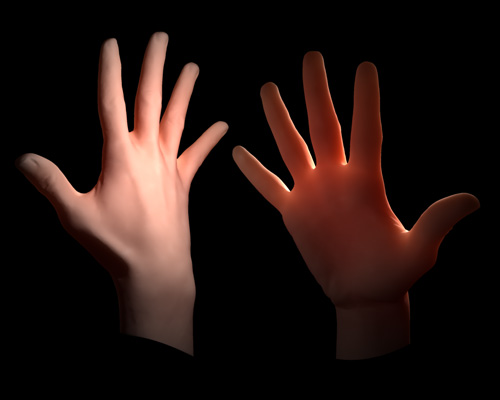
\includegraphics[width=9cm]{figuras/subsurface}}
	}{
		\Fonte{\url{http://www.mrbluesummers.com/wp-content/uploads/2010/07/Sub-Surface-Scattering-Example.jpg}}
	}
\end{figure}
\nocite{subsurface}

A escolha final das game engines requer a ponderação de alguns fatores como tipo de licensa, possibilidade de modificação do código, possível uso comercial, especificações de hardware, plataforma alvo, habilidade da equipe de desenvolvimento, ferramentas de suporte, estabilidade da engine e público alvo \cite{navarro2012}.

Por serem ferramentas complexas, sua comparação é uma tarefa complicada. A maneira mais apropriada seria implementar o mesmo projeto com complexidade apropriada e de maneira similar em cada game engine utilizando critérios mensuráveis para avalização \cite{vsmid2017comparison}.  

\subsection{Godot}
\label{sec:godot}



\subsection{Unity}
\label{sec:unity}

Unity é um motor de jogo desenvolvido e mantido pela empresa Unity Technologies que permite a criação de jogos 2D e 3D. Apesentada em 2005, sua primeira versão era simples e compatível apenas com Mac OS, porém com sua evolução foi adicionado suporte a outras plataformas (PC, Linux, Android, iOS, PS4, etc) \cite{compStudyGE}. Esse foi um dos principais fatores que tornou essa engine tão popular. Já que por suportar mais plataformas, pode proporcionar acesso a um público mais amplo.

Ela faz uso do DirectX como pipeline de renderização padrão, mas além disso ela utiliza quatro atividades de renderização adicionais. A pipeline de renderização direta é dividida em passagem de ambiente para objetos não afetados pela luz, passagem de transparência e passagem de luz para objetos opacos. Já a pipeline de renderização diferida é baseada em um modelo inteligente que primeiro computa a geometria e depois aplica a luz \cite{simon2015unity}.

A pipeline de renderização de pré-passagem é direcionada para as restrições no uso de diferentes shaders no processo diferido. As informações de luz são guardadas em um buffer para melhorar a performance dos cálculos. Por último é realizado o processo de renderização de vértices iluminados (cada objeto é renderizado com a iluminação de todas as fontes de luz calculada nos vértices) que é o mais rápido \cite{simon2015unity}. 

Sua arquitetura consiste em um sistema modular baseado em componentes que são utilizados para compor os objetos nos jogos. Cada componente possui um conjunto de funcionalidades que afetam o comportamento do objeto, dessa forma não é necessário usar herança. Isso é uma vantagem visto que aumenta a flexibilidade e a eficiência da modificação dos objetos \cite{compStudyGE}.

Cabe ainda destacar que ela possui uma das melhores documentações. A maioria das funções são descritas em profundidade e com bastante uso de exemplos, o que é muito útil principalmente para usuários iniciantes. Além disso ela possui uma vasta quantidade de templates, uma interface limpa e fácil de configurar, uma comunidade ativa, e seu uso de C\# ao invés de C++ torna a programação mais simples e agradável \cite{compStudyGE}.

Conforme verificado em estudo por Costa, Gomes, Duarte (2016)\nocite{estudoUnity}, dentre os motores de jogo a Unity é uma das ferramentas mais vantajosa do ponto de vista de produção por possuir um formato mais profissional e comercial, voltado para desenvolvimento multiplataforma. Além disso ela é capaz de performar melhor em composições de hardware mais simples.

A escolha da Unity pode-se justificar pelo fato de sua notável popularidade e seu crescimento constante, sendo que mais de 47\% dos desenvolvedores de jogos utilizam-na, com aproximadamente 45\% de participação no mercado de game engines e mais de 600 milhões de jogadores gastando mais de US\$ 110 bilhões \cite{simon2015unity}.

Na Unity os shaders são escritos em uma linguagem descritiva chamada \textit{ShaderLab}. Entretanto, o código do shader em si é escrito em HLSL. Ela oferece suporte a alguns tipos de shaders: de superfície (facilita a interação com luz e sombra), de vértice e de fragmento e de funções fixas \cite{aino2020}.

Há ainda alguns shader mais complexos que conseguem modificar a geometria base de malhas. São os shaders de geometria e tesselação, que pode ser utilizados para adaptar a qualidade visual ao nível de detalhe exigido por meio da otimização da malha em tempo real conforme sua distância da câmera \cite{aino2020}.

\subsection{Unreal}
\label{sec:unreal}

Unreal é mais um motor de jogo que está a mais tempo no mercado (desde 1998). Ela também permite a criação de jogos para múltiplas plataformas. Ela possui uma ferramenta específica para criação de scripts chamada \textit{BluePrint} que permite implementar lógica de programação usando blocos, porém também é possível criar scripts em C++ \cite{compStudyGE}.

\begin{figure}[h!]
	\centering
	\Caption{\label{fig:blueprint} A programação da lógica do jogo pode ser feita utilizando o sistema visual de \textit{BluePrint}.}	
	\UNIFORfig{}{
		\fbox{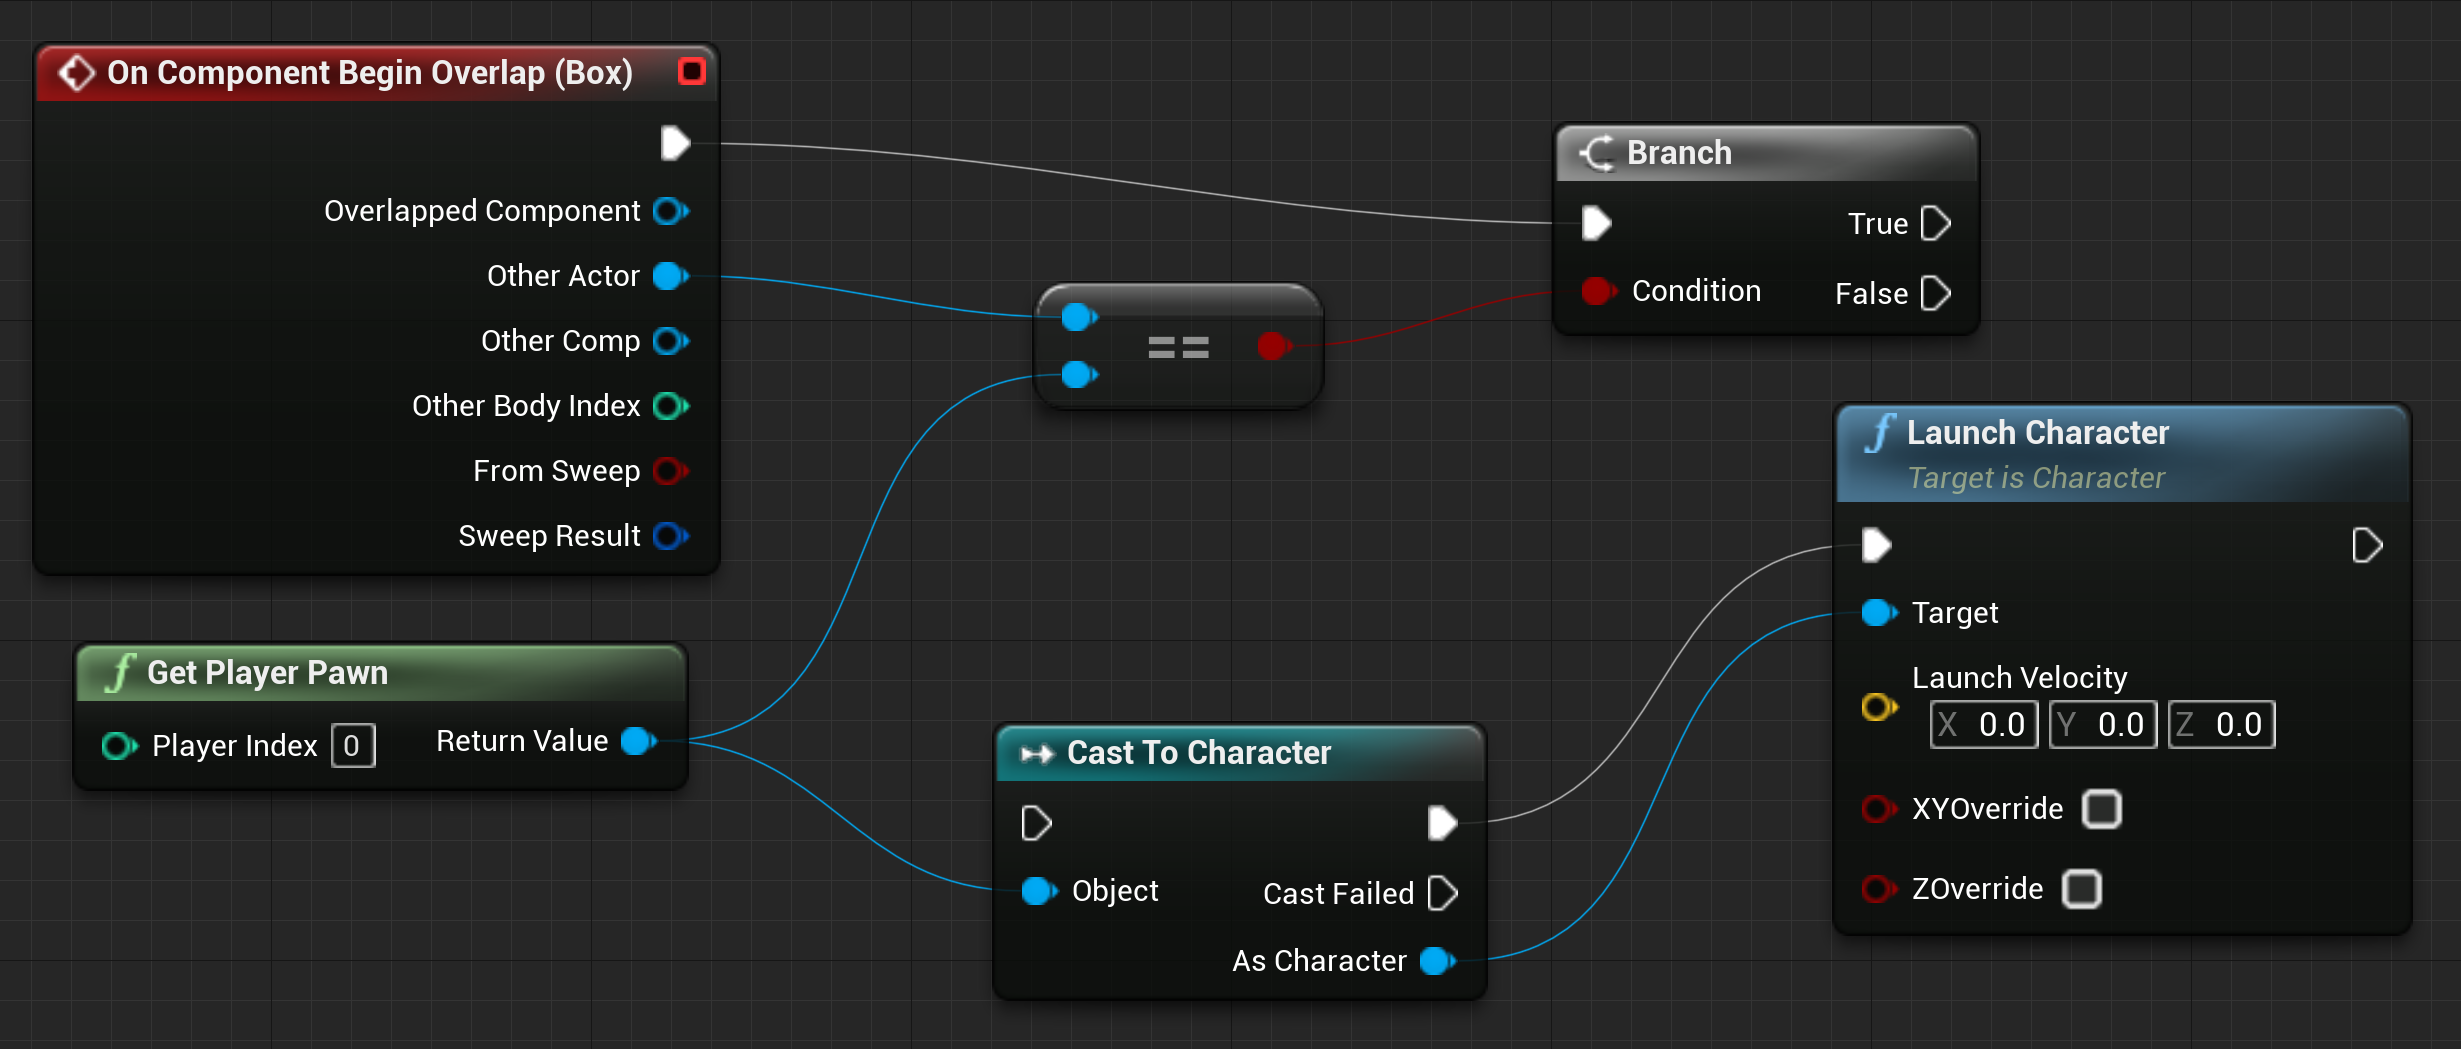
\includegraphics[width=14cm]{figuras/blueprint}}
	}{
		\Fonte{\url{https://docs.unrealengine.com/4.27/Images/ProgrammingAndScripting/Blueprints/QuickStart/BPQS_6_Step4.png}}
	}
\end{figure}
\nocite{blueprint}

É uma engine, em comparação com a Unity, mais difícil de dominar apesar de possui uma interface amigável, porém com excesso de opções à primeira vista. Seu sistema de programação com \textit{BluePrints} (Figura \ref{fig:blueprint}) traz uma vantagem para pessoas que não sabem ou não gostam de escrever código \cite{compStudyGE}.

Merecem destaque seu sistema de renderização \Gls{multithread} (intitulado Gemini) com 64 bits de HDR (\acrlong{HDR}), oclusão de ambiente, iluminação por pixel, iluminação especular dinâmica e reflexões, seu sistema de customização de terrenos e ainda o sistema de malhas de navegação para integração com personagens controlados por inteligência artificial \cite{armstrong2013game}.

Unreal apresenta uma melhor performance audiovisual de maneira geral. Além disso ela apresenta uma interface mais complexa em comparação com Unity e Godot que oferece todas as ferramentas necessárias em uma única janela. É portanto uma engine voltada para usuários mais experientes e hardwares mais robustos \cite{stelios2017}.

Essa engine 
 
\subsubsection{Nós de material}
\label{sec:material-nodes}

Unreal provê uma ferramenta de edição visual de grafos de nós para definição de expressões que computam parâmetros de entrada para modelos de materiais pré-definidos pela engine. Cada nó na expressão do grafo corresponde a um \textit{snippet} (pequeno pedaço de código) de shader que é composto com código modelo de material provido pela própria engine durante a compilação \cite{he2016rapid}.

Novamente a Unreal se destaca, por implementar uma ferramenta visual de edição de materiais que reutiliza os nós das \textit{BluePrints} mencionadas anteriormente, porém dessa vez voltadas para a modificação das propriedades dos materiais, o que torna o processo de criação de shader bastante amigável e divertido por estimular visualmente a criatividade dos usuários \cite{compStudyGE}. 

\begin{figure}[h!]
	\centering
	\Caption{\label{fig:materialUnreal} Uso de uma textura como base para definir a cor de um material.}	
	\UNIFORfig{}{
		\fbox{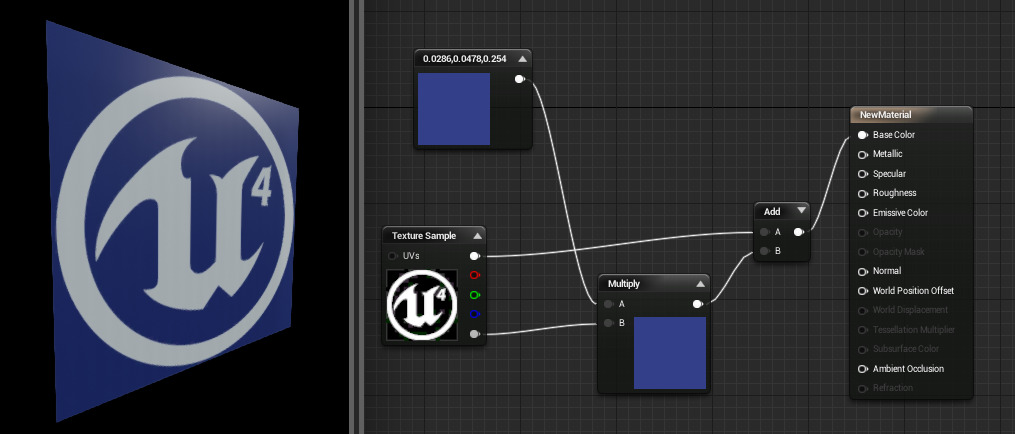
\includegraphics[width=13cm]{figuras/materialUnreal}}
	}{
		\Fonte{\url{https://docs.unrealengine.com/4.27/Images/RenderingAndGraphics/Materials/PhysicallyBased/BaseColor_QS.webp}}
	}
\end{figure}
\nocite{materialUnreal}

Seu sistema de materiais é uma das melhores ferramentas. Para cada material é compilado um shader. Então é possível utilizar o mesmo material ou pequenas variações deste. Esse método proporciona aos artistas uma ferramenta poderosa para criação de materiais, porém o lado negativo é que no caso de shaders mais complexos o tempo de compilação pode aumentar bastante \cite{vsmid2017comparison}.

Por baixo dos panos, essa engine implementa uma otimização de sombreamento chamada cascata de sombras. Ela renderiza múltiplos mapas de sombra baseado na distância da câmera para que objetos mais próximos tenham sombras mais definidas que objetos distantes. Há uma mistura suave entre esses mapas para que a mudança seja quase imperceptível. Isso melhora a performance e é muito eficiente especialmente para grandes cenas \cite{vsmid2017comparison}. 

\section{Otimização e performance}
\label{sec:otimizacao-performance}

Embora as arquiteturas de shaders forneçam execuções rápidas, a avaliação de shaders gera um custo alto no processo de renderização. Para shaders grandes (como os usados em filmes) pode igualar e exceder os custos associados com remoção de superfícies ocultas e processamento de geometria \cite{fabio2005user}. 

Isso torna-se um problema ainda maior em aplicações de tempo real que possuem restrições rígidas de taxa de quadros. Nesse caso, a simplificação geométrica é constantemente utilizada para fornecer um forma de compensação entre a qualidade da imagem percebida e a velocidade de execução em relação ao tamanho da malha do objeto \cite{fabio2005user}.

Cabe ressaltar que para \citeauthoronline{riguer2002performance} (2002), a performance média de um sistema e tão boa quanto o desempenho no pior gargalo. Então a tarefa de otimização pode ser reduzida à encontrar o pior gargalo e removê-lo (ou amenizá-lo). Esse é um processo iterativo que deve ser repetido até que o desempenho esteja em um limite aceitável.

Um gargalo de largura de banda de memória pode ocorrer quando há uso intenso de dados de vértices dinâmicos, uma solução seria reduzir a transferência de dados dinâmicos ou diminuir o tamanho de vértice. Já um gargalo de componente gráfico pode ser causado pelo próprio sistema \cite{riguer2002performance}.

Continuando, quando há cálculos por vértice ou uso de luzes em excesso pode ocorrer um gargalo de processamento de vértices. Por outro lado, o uso de shaders de fragmento complexos também pode gerar um gargalo. Além disso, o excesso de pixels renderizados por segundo pode gerar um gargalo de taxa de preenchimento \cite{riguer2002performance}.

Outrossim, o uso de texturas de alta definição e de filtros complexos pode acarretar em um gargalo de carregamento de textura. Por fim, o uso excessivo de recursos de transparência, profundidade e amostragem pode causar um gargalo no processo de rasterização. Na maioria das vezes o que se percebe é uma combinação de vários gargalos atuando em conjunto \cite{riguer2002performance}. 

Enquanto é considerada uma prática comum usar geometria dinâmica, não é bom abusar. Uma quantidade muito maior de polígonos pode ser obtida com geometria estática. Transformar geometria dinâmica em estática e aproveitar shaders de vértice para mover animações para a GPU pode ajudar a balancear a carga de trabalho \cite{riguer2002performance}. 

Devido à sua natureza de operação que requer simulação em tempo real, os jogos eletrônicos são softwares que exigem bastante recursos de hardware. Ainda mais atualmente quando os desenvolvedores cada vez mais objetivam criar produtos que perfaçam 60 frames por segundo (FPS) ou mais. Dessa forma, para atingir o maior público possível, vale a pena usar ferramentas que possibilitem o uso mais otimizado possível desses recursos \cite{comparacaoDesempenho}.

Com o crescimento do mercado de dispositivos móveis, a oportunidade de desenvolver e vender aplicações sofisticadas para esses dispositivos é ainda mais atrativa. Entretanto há também uma enorme quantidade de desafios ao lidar com esse tipo de tecnologia, entre eles: fonte de alimentação, quantidade de poder computacional, tamanho do display e tipos de entrada. Além disso, os processadores de smartphones não tratam números de ponto flutuante, o que reduz muito a precisão dos cálculos \cite{optimizationMobile}.

Na GPU de dispositivos móveis o número de espaços de instrução é limitado para os shaders de vértice e fragmento. Enquanto empacotar múltiplos ciclos de renderização em um único shader de fragmento aumenta a contagem de instruções, aumentar a quantidade de ciclos de renderização diminui o fracionamento paralelo. Nesse caso a melhor solução dependerá das necessidades da aplicação \cite{designMobileGPU}. 

Segundo Singhal et al. (2011) algumas formas de otimizar shaders seriam por meio de compressão de texturas para diminuir a sobrecarga de transferência de memória (ou utilizar um formato de pixel de menor precisão), pré-computar coordenadas vizinhas de texturas no shader de vértice e substituir laços por códigos otimizados ou utilizar vetores para realizar operações (diminuir a quantidade de instruções).

Considerando o trabalho de \citeauthoronline{nusrat2021commit} (2021), cabe aos desenvolvedores simplificar os gráficos para melhorar a performance. Simplificação de shaders e de modelos 3D são os tipos de melhorias mais comuns que podem afetar a experiência visual dos usuários. Por exemplo, ativar o corte de oclusão estático/dinâmico desativa a renderização de objetos cobertos e ativar o \Gls{light-baking} pré-calcula efeitos de luz durante a compilação.

Nesse sentido, os desenvolvedores devem tentar entender o custo computacional dos shaders e modelos 3D antes de usá-los. Para isso, antes de adicioná-los, devem ser feitos testes pois ao inserir vários modelos e shaders pode ser difícil distinguir quais estão causando problemas de performance \cite{nusrat2021commit}.

Devido a melhoria no poder de processamento gráfico, o uso de técnicas como iluminação 3D, vegetação gerada proceduralmente e fotogrametria aumentou consideravelmente tornando o processo de renderização mais custoso. Métodos comuns para otimização de cenas que fazem uso dessas técnicas são alocação de memória, \Gls{multithread}, e nível de detalhe. Ou seja, realizar a renderização em uma thread separada da lógica do jogo ajuda bastante a melhorar a performance \cite{zhang2017vegetation}.

Nível de detalhe é uma forma de determinar a distribuição dos recursos de renderização entre os objetos (de acordo com a posição e a importância atribuída aos vértices desses), diminuindo o número de dados desnecessários. Outrossim, são gerados modelos simplificados que reduzem a complexidade da cena e permitem uma renderização em tempo real mais eficiente \cite{zhang2017vegetation}.

Como as GPUs normalmente possuem ótima capacidade de processamento de vértices, a etapa de sombreamento de vértices raramente gerará um gargalo. Entretanto quando muitos pixels precisam ser processados por um shader de fragmentos com muitas instruções é esperado que haja um gargalo. Pode-se dizer que o número de instruções é inversamente proporcional à performance (taxa de frames) \cite{optimizationMobile}.

O controle de precisão de ponto flutuante --- em OpenGL baixo (10 bits), médio (16 bits) e alto (32 bits) --- é uma ótima ferramenta para melhorar o desempenho, porém precisa ser usada de forma apropriada, pois um nível de baixa precisão apesar de melhorar a performance pode acabar gerando artefatos indesejados \cite{optimizationMobile}.

\begin{table}[h!] 
	\centering
	\Caption{\label{qua:instrucoes} Número de instruções necessárias para operações específicas no OpenGL}\UNIFORqua{}{
	\begin{tabular}{|c|p{2cm}|p{2cm}||c|p{2cm}|p{2cm}|}
	\hline
	Operação & Número de Instruções & Número de ciclos de renderização & Operação & Número de Instruções & Número de ciclos de renderização \\
	\hline
	\begin{tabular}[c]{@{}c@{}}
		RGB2GRAY\\ RGB2YCbCr\\ YCbCr2RGB\\ RGB2HSV\\ HSV2RGB\\
	\end{tabular} &
	\multicolumn{1}{c|}{
	\begin{tabular}[c]{@{}c@{}}
		5\\ 14\\ 14\\ 28\\ 29\\
	\end{tabular}} &
	\multicolumn{1}{c||}{
	\begin{tabular}[c]{@{}c@{}}
		1\\ 1\\ 1\\ 1\\ 1\\
	\end{tabular}} &
	\begin{tabular}[c]{@{}c@{}}
		Gaussian \\Sharpening \\Gradient \\Bilateral \\Laplacian \\Box filter\\
	\end{tabular} &
	\multicolumn{1}{c|}{
	\begin{tabular}[c]{@{}c@{}}
		21\\ 13\\ 19\\ 62\\ 14\\18\\
	\end{tabular}} &
	\multicolumn{1}{c|}{
	\begin{tabular}[c]{@{}c@{}}
		1\\ 1\\ 2\\ 2\\ 1\\1\\
	\end{tabular}} \\
	\hline
	\begin{tabular}[c]{@{}c@{}}
		Bloom\\ Skin detection\\
	\end{tabular} &
	\multicolumn{1}{c|}{
	\begin{tabular}[c]{@{}c@{}}
		15\\ 25
	\end{tabular}} &
	\multicolumn{1}{c||}{
	\begin{tabular}[c]{@{}c@{}}
		1\\ 2
	\end{tabular}} &
	\multicolumn{1}{c|}{
	\begin{tabular}[c]{@{}c@{}}
		Sobel \\Prewitt
	\end{tabular}} &
	\multicolumn{1}{c|}{
	\begin{tabular}[c]{@{}c@{}}
		24\\ 16
	\end{tabular}} &
	\multicolumn{1}{c|}{
	\begin{tabular}[c]{@{}c@{}}
		2\\ 2
	\end{tabular}} \\
	\hline
	\begin{tabular}[c]{@{}c@{}}
		Detail enhancement \\Edge enhancement
	\end{tabular} &
	\multicolumn{1}{c|}{
	\begin{tabular}[c]{@{}c@{}}
		13\\ 25
	\end{tabular}} &
	\multicolumn{1}{c||}{
	\begin{tabular}[c]{@{}c@{}}
		1\\ 2
	\end{tabular}} &
	\multicolumn{1}{c|}{
	\begin{tabular}[c]{@{}c@{}}
		Contrast Stretching \\Median filtering
	\end{tabular}} &
	\multicolumn{1}{c|}{
	\begin{tabular}[c]{@{}c@{}}
		13\\ 43
	\end{tabular}} &
	\multicolumn{1}{c|}{
	\begin{tabular}[c]{@{}c@{}}
		1\\ 1
	\end{tabular}} \\ 
	\begin{tabular}[c]{@{}c@{}}
		Dilation \\Median
	\end{tabular} &
	\multicolumn{1}{c|}{
	\begin{tabular}[c]{@{}c@{}}
		22\\ 43
	\end{tabular}} &
	\multicolumn{1}{c||}{
	\begin{tabular}[c]{@{}c@{}}
		1\\ 1
	\end{tabular}} &
	\multicolumn{1}{c|}{
	\begin{tabular}[c]{@{}c@{}}
		Erosion \\Zero-crossing
	\end{tabular}} &
	\multicolumn{1}{c|}{
	\begin{tabular}[c]{@{}c@{}}
		22\\ 22
	\end{tabular}} &
	\multicolumn{1}{c|}{
	\begin{tabular}[c]{@{}c@{}}
		1\\ 1
	\end{tabular}} \\
	\hline
	\begin{tabular}[c]{@{}c@{}}
		Sepia \\Radial Blur \\Edge overlay \\Gray
	\end{tabular} &
	\multicolumn{1}{c|}{
	\begin{tabular}[c]{@{}c@{}}
		21\\ 21\\ 25\\ 5
	\end{tabular}} &
	\multicolumn{1}{c||}{
	\begin{tabular}[c]{@{}c@{}}
		1\\ 1\\ 2\\ 1
	\end{tabular}} &
	\multicolumn{1}{c|}{
	\begin{tabular}[c]{@{}c@{}}
		Color gradient\\Negative\\Gamma\\Edge
	\end{tabular}} &
	\multicolumn{1}{c|}{
	\begin{tabular}[c]{@{}c@{}}
		20\\ 2\\ 15\\ 24
	\end{tabular}} &
	\multicolumn{1}{c|}{
	\begin{tabular}[c]{@{}c@{}}
		1\\ 1\\ 1\\ 2
	\end{tabular}} \\ \hline  
	\end{tabular}
	}{
		\Fonte{\citeauthoronline{optimizationMobile} (2010)}
	}
	\end{table}

Para \citeauthoronline{lewis2018evaluation} (2018), a quantidade de linhas de código de um shader segue um distribuição de lei de potência, com poucos shaders longos, e vários shaders simples (poucas linhas). Entretanto, até os shaders mais longos possuem em torno de 300 linhas. A maioria contém menos que 50 linhas. Isso mostra que normalmente shaders são bem menores que softwares.

Além disso, como o número de vértices processados em operações de processamento de imagens é muito mais baixo que o de fragmentos (podem ser da ordem de milhões), é recomendado realizar cálculos por vértice ao invés de por fragmento por aquelas serem menos custosas. Por fim, cabe salientar que maiores velocidades de clock favorecem a performance \cite{optimizationMobile}.

Como a criação de jogos tornou-se mais acessível, vários jogos são criados e lançados frequentemente. Com o aumento da quantidade de jogos no mercado os desenvolvedores precisam fazer com que eles se destaquem da concorrência. Para isso é comum o uso de modelos gráficos com muitos detalhes, o que pode acabar sobrecarregando o sistema significativamente \cite{performanceTesselation}. 

Quando muitos deles estão presentes na tela ao mesmo tempo, o jogo pode não funcionar bem, e isso afeta negativamente a experiência dos jogadores. Uma solução para esse problema consiste em aplicar algoritmos de tesselação para substituir dinamicamente modelos de objetos presentes no jogo. Cada modelo é substituído por um mais simplificado conforme a câmera se afasta, reduzindo a carga no sistema \cite{performanceTesselation}.

A maioria dos motores de jogos disponíveis no mercado oferecem uma ferramenta para geração automática de níveis de detalhe para modelos 3D. A única coisa que o desenvolvedor do jogo deve fazer é indicar como os níveis de detalhe devem ser gerados (caso os parâmetros padrões não se adequem ao seu projeto). A Unreal Engine possui uma ferramenta embutida para gerar níveis de detalhe por padrão com várias configurações prontas preparadas pelos criadores. A ferramenta é capaz de gerar automaticamente o número apropriado de níveis de detalhe \cite{performanceTesselation}.

Uma forma de otimização de shaders já descrita por Rost (2006) consiste na substituição da função de ruído embutida na linguagem de shader por uma função criada pelo próprio desenvolvedor ou por uma textura. A última opção é a melhor em termos de performance. Felizmente, a programabilidade oferecida pela GLSL torna possível pré-computar uma função de ruído e salvar seu resultado em mapas de textura de uma, duas ou três dimensões em cada um de seus quatro componentes.

Outra técnica útil para melhorar a performance ao lidar com várias luzes é o sombreamento diferido, que basicamente determina quais superfícies serão visíveis na cena final e aplica cálculos complexos de efeitos de shader apenas nos pixels que compõem essas superfícies. Dessa maneira, as operações são adiadas até que sejam estabelecidos os pixels que contribuirão para a imagem final. Essa técnica garante que não haja desperdício de ciclos de hardware com cálculos em pixels que sequer serão exibidos na tela \cite{GLSLBook}.

Mais uma maneira de otimização descrita por Jensen \textit{et al}. (2007) seria garantir que o código de shader seja movido para sua parte menos custosa. Nesse caso existem três possíveis lugares: no programa de vértices, no programa de fragmentos, ou nas declarações constantes. A última é a mais otimizada pois os cálculos são realizados em tempo de compilação. A segunda forma mais otimizada seria utilizar o espaço do programa de vértices, mas se houver muito código nessa parte haverá um desbalanceamento.

Caso seja necessário realizar transformações de coordenadas a melhor opção seria utilizar o espaço do programa de vértices (por exemplo mover transformação da direção da luz em espaço tangente para essa etapa). Ao ponderar-se esses detalhes para as ferramentas de criação de shaders visuais, percebe-se que há uma certa dificuldade em realizar otimizações manuais, já que o código é gerado automaticamente \cite{jensen2007shader}.

Um dos erros mais comuns é usar texturas muito grandes desnecessariamente, o que prejudica bastante a performance, sendo que alguns objetos nunca atingem um tamanho grande na tela. O ideal seria tentar utilizar texturas com dimensões que não são potências de dois para diminuir o consumo de memória. Além disso, deve-se evitar a troca excessiva de texturas \cite{riguer2002performance}.

Segundo \citeauthoronline{arnau2014} (2014), uma possível técnica de otimização seria o uso de memoização para evitar a execução redundante de computações reutilizando resultados anteriores, o que resulta em aumento de velocidade de execução e economia de energia. De forma simplificada, os cálculos realizados são salvos em uma tabela para que no próximo cálculo os valores sejam reutilizados.

\citeauthoronline{he2016rapid} (2016) define o processo de otimização em várias etapas: identificação de componentes de shaders que podem ser transformados em texturas, uso de pré-processamento \textit{offline} para os buffers de parâmetros, seleção da melhor frequência espacial ou espaço de coordenadas para as funções e escolha de técnicas multi-resolução ou formas de reuso.

Esse é um desafio e tanto para game engines modernas, que podem conter vários shaders únicos, implementando uma vasta coleção de materiais e múltiplos níveis de detalhe --- por exemplo, o jogo Bungie’s Destiny usa mais de 17 mil materiais compilados para 180 mil shaders --- que podem exigir diferentes procedimentos de otimização \cite{he2016rapid}.

Para medir a performance, é necessária uma forma de \Gls{benchmark} para comparar a performance com mais precisão e objetividade. Alguma áreas onde o Benchmark é importante são na iluminação global, detecção de colisão, animação, renderização e em áreas onde é preciso medir e comparar a performance \cite{lext2001ray}.

Uma métrica muito comum para sistemas interativos de tempo real é a quantidade de quadros por segundo (taxa de quadros). Ela mede a frequência média de uma aplicação no hardware onde é executada. Assim pode-se obter diferentes valores para diferentes tipos de hardware. Essa é uma medida comum entre várias revistas de jogos de computadores para medir a performance \cite{rehfeld2014profile}.
